\documentclass[times, utf8, zavrsni, numeric]{fer}
\usepackage{booktabs}
\usepackage{listings}
\usepackage{xcolor}
\usepackage{graphicx}
\graphicspath{ {./notes/screenshots/} }

\colorlet{punct}{red!60!black}
\definecolor{background}{HTML}{EEEEEE}
\definecolor{delim}{RGB}{20,105,176}
\colorlet{numb}{black!60!black}

\lstdefinelanguage{json}{
    basicstyle=\normalfont\ttfamily,
    numbers=left,
    numberstyle=\scriptsize,
    stepnumber=1,
    numbersep=8pt,
    showstringspaces=false,
    breaklines=true,
    frame=lines,
    backgroundcolor=\color{background},
    literate=
     *{0}{{{\color{numb}0}}}{1}
      {1}{{{\color{numb}1}}}{1}
      {2}{{{\color{numb}2}}}{1}
      {3}{{{\color{numb}3}}}{1}
      {4}{{{\color{numb}4}}}{1}
      {5}{{{\color{numb}5}}}{1}
      {6}{{{\color{numb}6}}}{1}
      {7}{{{\color{numb}7}}}{1}
      {8}{{{\color{numb}8}}}{1}
      {9}{{{\color{numb}9}}}{1}
      {:}{{{\color{punct}{:}}}}{1}
      {,}{{{\color{punct}{,}}}}{1}
      {\{}{{{\color{delim}{\{}}}}{1}
      {\}}{{{\color{delim}{\}}}}}{1}
      {[}{{{\color{delim}{[}}}}{1}
      {]}{{{\color{delim}{]}}}}{1},
}
\lstset{
  language=bash,
  basicstyle=\ttfamily,
  breaklines=true,
  showstringspaces=false,
  numbers=left,
  stepnumber=1,
  numbersep=8pt,
  frame=lines,
  backgroundcolor=\color{background},
  numberstyle=\scriptsize
}

\begin{document}

% TODO: Navedite broj rada.
\thesisnumber{000}

% TODO: Navedite naslov rada.
\title{Usporedba performanci Ethereum raspodijeljene knjige na raznorodnom sklopovlju}

% TODO: Navedite vaše ime i prezime.
\author{Jakov Buratović}

\maketitle


% Dodavanje zahvale ili prazne stranice. Ako ne želite dodati zahvalu, naredbu ostavite radi prazne stranice.
\zahvala{Zahvaljujem se mentoru doc. dr. sc. Igoru Čavraku i kolegi Ediju Sinovčiću na podršci i pomoći pri izradi ovog rada.\\
Također se zahvaljujem i svojoj obitelji koja me usmjeravala i pomagala tokom preddiplomskog studija.
}

\tableofcontents

\chapter{Uvod}
\emph{Ethereum} mnogi znaju kao jednu od najpopularnijih kriptovaluta. Iako je to točno, \emph{Ethereum} je mnogo
više od same digitalne valute. To je programska potpora raspodijeljena na mreži računala na kojima je
moguće razmjenjivati podatke i pokretati računalne programe bez centralnog poslužitelja. 
Podaci se repliciraju na svaki čvor u mreži. Određenim algoritmima konsenzusa se osigurava 
nepromjenjivost i pouzdanost. 
To omogućuje da mreža bude potpuno javna i sigurna. Posebnost je što svatko može koristiti
mrežu i objavljivati sadržaj bez ikakvih posebnih dozvola. \\ Za razliku od \emph{Bitcoina}
i mnogih drugih implementacija tehnologije distribuirane knjige koji nude mogućnost pohrane podataka
bez centralnog poslužitelja, \emph{Ethereum} mreža omogućuje i izvođenje programskog koda u obliku pametnih ugovora.\\
U ovom radu je prikazano kako se može pokrenuti privatna mreža na različitom sklopovlju uz  ispitivanje najnižih zahtjeva sklopovlja.
Dodatno, prikazat će se proces obavljanja transakcija i izvođenja programskog koda na čvorovima uz prigodni prikaz sa sučeljem u jednostavnoj web aplikaciji.\\
U prvom poglavlju ovog rada, objasnit će se osnove tehnologije distribuirane knjige i njene primjene.\\
Nakon toga će biti poglavlje usmjereno na \emph{Ethereum} kao implementaciju navedene tehnologije algoritmom ograničenih skupova autoriziranih čvorova mreže (engl. \emph{Proof of Authority}). \\
Posljednje poglavlje je zaduženo za detaljan postupak kreiranja privatne mreže na raznorodnom sklopovlju
s različitim operativnim sustavima uz dodatak programske podrške za praćenje transakcija i stanja mreže.  

\chapter{Tehnologija glavne raspodijeljene knjige}
U nastavku ćemo tehnologiju glavne raspodijeljene knjige (engl. \emph{Distributed Ledger Technology})
 referencirati kraće po kratici engleskog naziva, odnosno DLT. \\ 
DLT i blockchain se često poistovjećuju no to nije u potpunosti ispravno. Bitno je znati da je 
svaki blockchain DLT s određenim pravilima konsenzusa.
DLT je baza podataka repliciranog sadržaja na svakom čvoru \emph{peer-to-peer} mreže. Svaki čvor
mora sadržavati identičnu kopiju kompletnog sadržaja baze podataka i konstantno se ažurira sa susjednim čvorovima. \\
Kod blockchaina se te promjene zapisuju u obliku transakcije u blokove koji formiraju neprekidan lanac.
Odatle dolazi i sam naziv tehnologije. Čvor koji upisuje transakciju u blok prvo sam provjeri njenu ispravnost pa je onda odašilje povezanim čvorovima.
Čvorovi koji primaju novu transakciju potrvđuju njenu valjanost i uključuju ju u idući blok. Prije nego što se novi blok transakcija poveže u postojeći lanac
blokova, on mora biti potvrđen od većine čvorova prema poznatim pravilima konsenzusa koji se koristi
u toj implementaciji mreže. Nakon što je blok povezan, sve transakcije zabilježene ostaju zauvijek i
šanse za maliciozne izmjene su vrlo malene. To su dvije najvažnije karakteristike DL tehnologije, konačnost (engl. \emph{finality}) i nepromjenjivost \emph{immutability}.

\section{Proof of work}
Prvi algoritam konsenzusa koji se koristio u \emph{blockchain} tehnologiji je bio \emph{proof of work},
 odnosno algoritam u kojem izvršeni rad procesora i utrošena električna energija
garantira svojstvo konačnosti i nepromjenjivosti. Izvorni primjer ove implementacije je \emph{Bitcoin}. \\
\emph{Bitcoin} je najpoznatiji primjer primjene blockchaina u široj populaciji. Njegova mreža je aktivna 
od siječnja 2009. godine kada je Satoshi Nakamoto potvrdio prvi blok (engl. \emph{genesis}).
Još uvijek nije poznato tko je Satoshi Nakamoto i je li to uopće stvarna osoba ili naziv za grupu
ljudi koji su sudjelovali u razvoju \emph{bitcoina}. Problem koji \emph{bitcoin} pokušava riješiti je centraliziranost
ekonomskog sustava i plaćanja. Svaka transakcija u trenutnom sustavu mora proći kroz centralno sjedište,
odnosno banku. To znači da korisnici moraju vjerovati centralnom sjedištu da će provesti transakcije
kako korisnik želi i da se neće ponašati maliciozno. Također, korisnici moraju vjerovati u sigurnost
centralnog sjedišta i mogućnost zaštite od napada od treće strane. \\
Za takav način je potreban velik broj ljudi, novca i kontrole što dovodi dodatna ograničenja kao što 
su čekanje na potvrdu transakcije dulje vrijeme, nemogućnost obavljanja transakcija vikendom i praćenje
toka novca. \\
\emph{Bitcoin} te probleme rješava tako da izbacuje centralno sjedište i umjesto njega koristi \emph{Proof of Work}
pravila konsenzusa koja osiguravaju pouzdanost bez povjerenja. \\
Nakon \emph{bitcoina} su se pojavili mnogi \emph{forkovi} s manjim ili većim promjenama, obično u veličini
samih blokova ili brzini potrvrđivanja istih. Oni su obilježili prvu generaciju kriptovaluta. \\
Kako bi se osigurala nepromjenjivost, računa se sažetak (engl. \emph{hash}) duljine 64 znaka sadržaja blokova. 
Svaki idući blok u izračunu svog sažetka koristi sažetke svih prijašnjih blokova u lancu i nasumični broj (engl. \emph{nonce}). Nasumični broj se inkrementira od 0
dok njegova vrijednost u kombinaciji sa sažetcima prijašnjih blokova ne da novi sažetak s ciljanim brojem nula na početku. Taj posao obavljaju validatori, poznati pod nazivom
rudari (engl. \emph{miners}). Primjer pogađanja je vidljiv na iduće dvije skice \citep{PoWAsync}. Prvi izračun koristi \emph{nonce} vrijednosti 1 i daje sažetak s vodeće
tri nule što ne odgovara trenutnom zahtjevu mreže.

\begin{figure}[ht]
  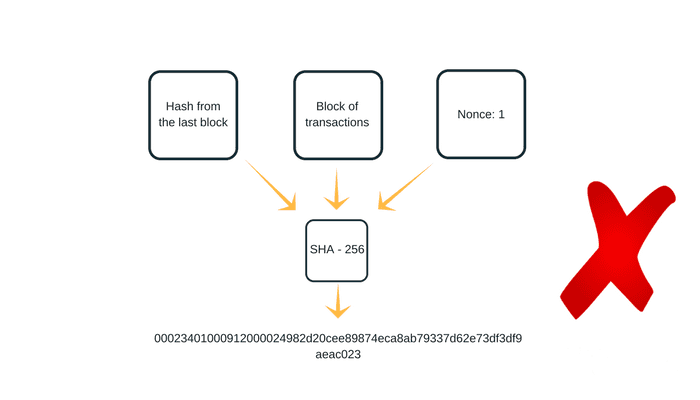
\includegraphics[width=\textwidth]{proof-of-work-wrong-result-2.png}
  \caption{Neuspjeli pokušaj}
  \centering
\end{figure}

U idućem koraku se vrijednost \emph{nonce} povećava za jedan što daje ispravno rješenje. Čvor koji je prvi došao do rješenja problema objavljuje svoj rezultat rada mreži
i za to dobiva nagradu u valuti čije transakcije potvrđuje. Ta nagrada je povod koji ljude privlači da troše resurse kako bi potvrđivali transakcije. Nagrada se sastoji
od unaprijed određene količine novčića, primjerice \emph{Bitcoina} i provizijama transakcija u bloku koji je potvrdio. 

\begin{figure}[ht]
  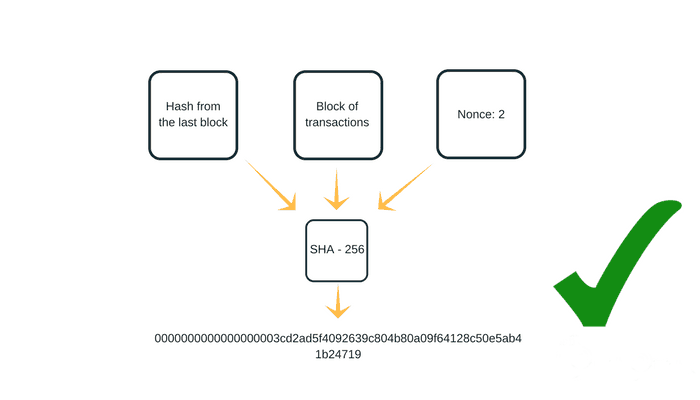
\includegraphics[width=\textwidth]{proof-of-work-right-result-2.png}
  \caption{Pogodak!}
  \centering
\end{figure}

Broj znamenaka nula se određuje težinom rudarenja. U \emph{Bitcoin} mreži se cilja da vrijeme između dva bloka bude oko 10 minuta.
Ako je u mreži puno rudara i ukupna procesorska snaga je visoka oni će pogoditi sažetak prije tog vremena što rezultira povećanjem vodećih nula za računanje idućih sažetaka. 
Isto tako, ako u mreži nema dovoljno procesorske snage za pogađanje, zahtjevnost pada i broj vodećih nula sažetka se smanjuje. 
Najmanja promjena u bilo kojem bloku ili transakciji u cijelosti mijenja sažetak te bi za uspješno izvršavanje maliciozne radnje
trebalo ponovno pogađati sve sažetke od izmijenjenog bloka i sustići glavni lanac. Pravilo je da uvijek najdulji lanac ostaje i novi blokovi transakcija se nadovezuju na njega.
Kako bi maliciozni korisnik uspio sustići glavni lanac svojim izmijenjenim blokovima i sažetcima mora imati preko 51\% ukupne procesorske snage cijele mreže rudara.
U nekim manjim mrežama je to lakše moguće izvesti, no u mreži \emph{Bitcoina} je to vrlo neisplativo jer je ukupna procesorska snaga i utrošak električne energije vrlo visok.
To je ujedno i glavni nedostatak ovog algoritma. Kako bi se osigurala sigurnost, troši se izrazito velika količina novca i rješenje nije ekološki povoljno.

\section{Proof of Stake}
Kako bi se riješio problem koji je imao \emph{PoW} algoritam, 2011. predloženo je novo rješenje u kojem se validiranje transakcija ne bi oslanjalo na utrošak električne energije
i procesorsku moć. U ovom algoritmu se nove blokove ne stvaraju rudari nego kovači (engl. \emph{forgers}). \\ Umjesto da se pouzdanost \emph{blockchaina} oslanja
na procesorsku moć i utrošenu električnu energiju u ovom algoritmu se gleda validatorov ekonomski ulog u mreži. Skup validatora naizmjenice predlažu
i glasaju za idući blok. Težina glasa validatora izravno ovisi o količini uloga. Prednosti ovog algoritma su sigurnost, smanjen rizik centralizacije i 
energijska efikasnost.\citep{PoSGithub}. \\
Kako bi čvor postao validator, potrebno je obaviti poseban tip transakcije kojim korisnik zaključava određeni ulog. Dok god je ulog zaključan, validator ima šansu
postati tvorac sljedećeg bloka. Uložena sredstva je moguće u bilo kojem trenutku otključati i ponovno koristiti za transakcije no time se gube glasovi tog validatora u mreži.
Kako bi se spriječila manipulacija mreže, nije dovoljno biti samo \emph{najbogatiji} u mreži već se gledaju i drugi kriteriji. Prvi je vrijeme proteklo od uloga tokena.
Validator čiji je ulog dulje zaključan ima veću šansu biti odabran kao sljedeći kovač bloka. Nakon što je validator stvorio blok, njegova duljina uloga se resetira kako
bi drugi validatori imali veću šansu postati kovači idućeg bloka.\citep{posMedium} \\
Primjer kako  odabrati kovača idućeg bloka je opisan u nastavku\citep{posGraphic}. 
\begin{figure}[ht]
  \centering
  \begin{minipage}[b]{0.49\textwidth}
    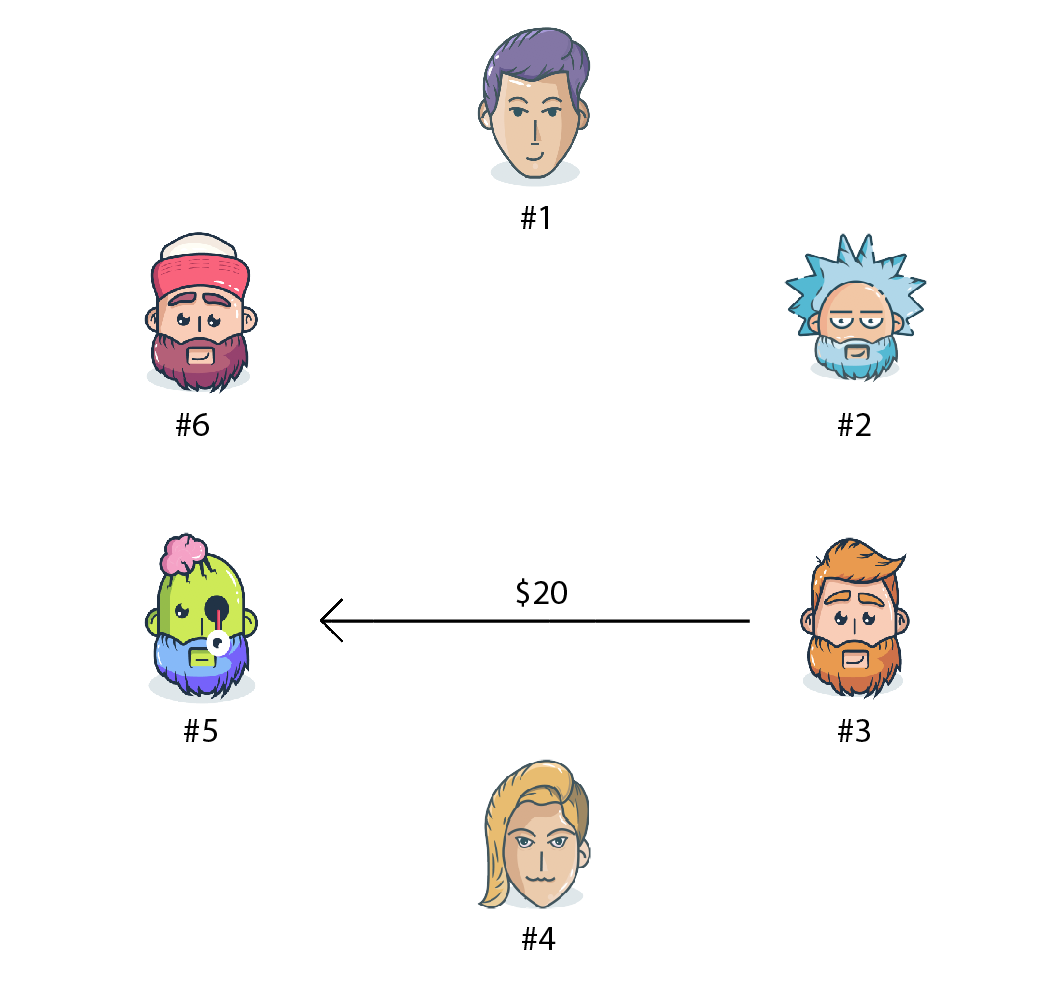
\includegraphics[width=\textwidth]{pos1.png}
    \caption{Transakcija}
  \end{minipage}
  \hfill
  \begin{minipage}[b]{0.5\textwidth}
    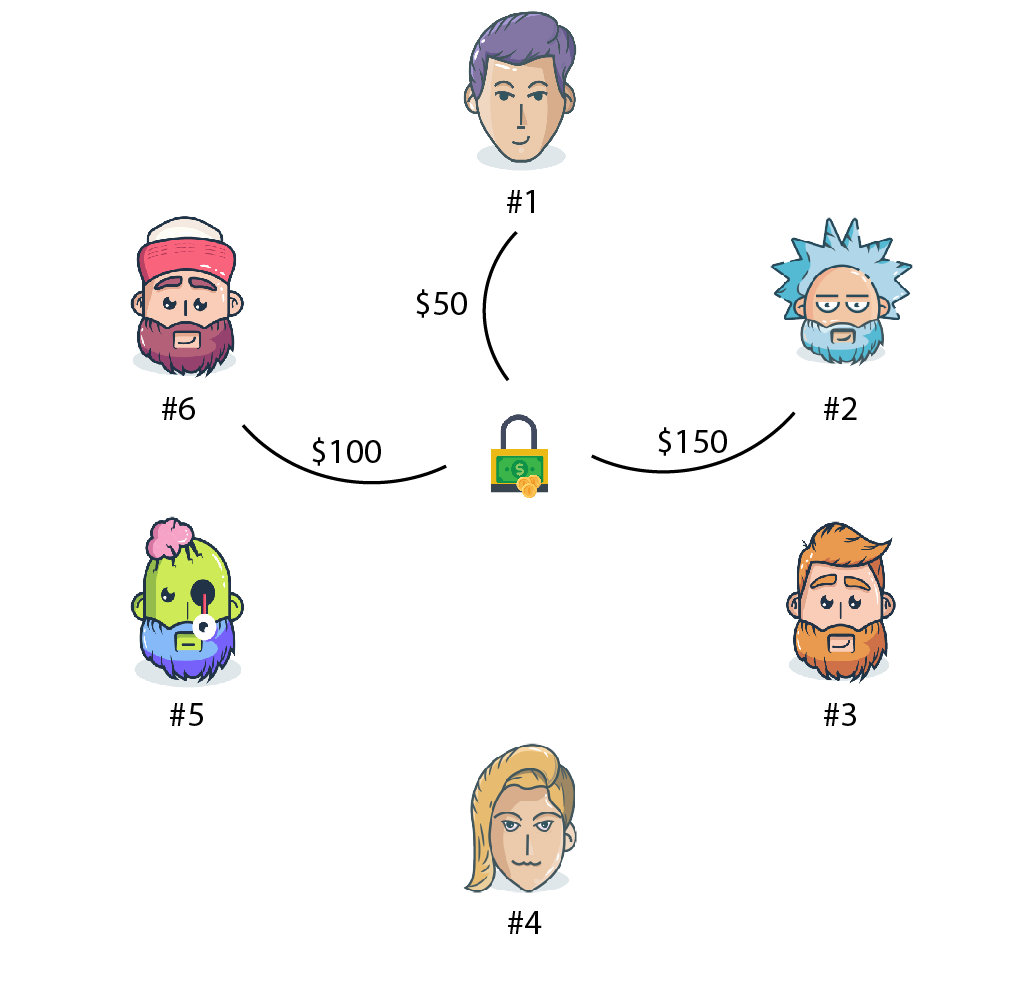
\includegraphics[width=\textwidth]{pos2.png}
    \caption{Biranje kovača}
  \end{minipage}
\end{figure}

\pagebreak
U ovom primjeru se pretpostavlja da je moguće imati samo jednu transakciju po bloku i da su svi članovi zaključali svoje tokene u isto vrijeme.
Na prvoj slici vidimo šest sudionika u mreži. Sudionik broj 3 šalje tokene vrijednosti 20 USD sudioniku broj 5. Tu transakciju treba uključiti u sljedeći blok kako bi bila valjana.
Sudionici broj jedan, dva i šest su uložili i svoje novce kako bi mogli postati kovačima. Ukupan ulog u mreži je 300 USD u tokenima. Kako su svi uložili tokene u isto vrijeme,
glavni faktor pri biranju kovača je količina zaključanih tokena. Sudionik broj 2 ima polovinu ukupnog uloga u mreži što mu daje čak 50\% šanse da postane kovač.
Sudionik broj 6 ima 33\% šanse dok broj 1 ima samo 17\% šanse da validaraju blok. Odabran je broj 2 koji mora provjeriti valjanost transakcije i uključiti blok u lanac.
Za to mu nije potrebno snažno računalo. Kao nagradu za validaciju transakcije je dobio proviziju koju je platio sudionik broj 3 prilikom slanja tokena. \\
Najveći problem u \emph{proof of stake} algoritmu je početna distribucija tokena. Kako količina tokena koju čvor posjeduje definira jačinu i važnost u mreži potrebno
je pronaći rješenje za taj problem. Jedno od rješenja je predložio \emph{Ethereum}, početi kao \emph{proof of work} mreža i s vremenom se prebaciti na \emph{proof of stake}.
To bi osiguralo ravnomjernu podjelu tokena rudarima i ostalim korisnicima mreže. Da bi rezultat tog procesa bio što bolji potrebno je mnogo vremena da se prirodnim 
tokom sredstava raspodijeli bogatstvo na velik broj novčanika. \\
Dodatno, ako validatori ne izvršavaju svoje dužnosti i potrđuju neispravne transakcije za to bivaju kažnjavani oduzimanjem uloženih tokena. Vrijednost uloženih tokena je
uvijek mnogo viša od nagrade za validiranje što znači da se sudionicima ne isplati riskirati ulog i varati.

\section{Proof of Authority}
\emph{Proof of Authority} ili dokaz o autoritetu jest modificiran oblik \emph{proof of stake} algoritma. Umjesto uloga novčane vrijednosti u tokenima, u ovom algoritmu
sam identitet validatora ima funkciju uloga. Identitet u ovom kontekstu znači pripadnost validatorove osobne identifikacije identitetu na platformi, odnosno
sigurnost da je validator osoba koja tvrdi da je. Kao i u \emph{PoS} algoritmu, identitet kao forma uloga je oskudan. No za razliku od njega, ovdje jedan identitet odgovara
jednoj osobi.\citep{poa1} \\
Samo potvrđeni identiteti mogu stvarati blokove. Nije potrebno ulagati tokene niti trošiti veliku količinu energije. Jedini zahtjev je da se identitet nalazi na listi
dopuštenih validatora. Ta lista može biti statična ili dinamična. Statična lista identiteta je definirana u specifikaciji prvog bloka \engl{genesis}. Nije moguće naknadno
izmijeniti tu listu. U drugom slučaju, listu je moguće izmijeniti tako da postojeći identiteti s liste dodaju nove ili brišu postojeće ako se oni ponašaju maliciozno.\citep{poa2} \\
Vrlo je lako primijetiti da ovaj način dopušta puno veću centraliziranost od preostalih algoritama konsenzusa. Iz tog mu razloga osnovna namjena nisu javne mreže nego manje mreže,
obično unutar nekih tvrtki ili zatvorenih sustava. U takvom okruženju nije bitno prikupljanje nagrada validiranjem transakcija pa su provizije najmanje moguće.
Osim niskih provizija, stvaranje novih blokova može biti vrlo brzo uz izrazito niske zahtjeve sklopovlja čvorova u mreži. Primjerice, testna mreža \emph{Ethereuma, Kovan}
radi na \emph{PoA} algoritmu i u njoj se novi blokovi stvaraju svakih 5 sekundi. To omogućava izvođenje programa kojima je važna brzina distribucije informacija po mreži. \\
Najpoznatija implementacija ovog algoritma je \emph{Clique}, dio službene \emph{Ethereum Geth} implementacije pisane u programskom jeziku \emph{Go}.
\emph{Clique} spada među implementacije u kojima se dinamički mogu mijenjati identiteti u listi. Skupovi blokova formiraju epohe. Nakon kraja svake epohe se objavljuje
poseban tranzicijski blok čiji je sadržaj nova lista autoriteta koji će imati ovlasti potpisivati i transakcije u idućoj epohi.

\chapter{Ethereum}
2013. godine ruski programer Vitalik Buterin predlaže \emph{Ethereum} svojim \emph{whitepaperom}\footnote{\url{https://ethereum.org/whitepaper/}}, novu javnu platformu koja koristi 
dorađeno izdanje Nakamotovog \emph{Proof of Work} konsenzusnog algoritma.
Od Buterinovog dokumenta do pokretanja \emph{Ethereuma} protekle su dvije prilično burne godine. Projekt je okupio nekoliko \emph{blockchain} stručnjaka, uključujući
Gavina Wooda, koji je definirao \emph{Ethereum} na tehničkoj razini u svom \emph{yellow paper} dokumentu\footnote{\url{https://ethereum.github.io/yellowpaper/paper.pdf}} te
izumio programski jezik \emph{Solidity}\footnote{\url{https://solidity.readthedocs.io/en/v0.6.9/}}, Charlesa Hoskinsona koji je na početku bio direktor projekta, Jeffreya
Wilkea, programera koji je izrazito puno doprinio projektu, te Josepha Lubina, koji je bio ključan u pokretanju zaklade \emph{Ethereum Foundation}
\footnote{\url{https://ethereum.foundation/}} u Švicarskoj.\citep{ffzg} \\
 \emph{Ethereum} je globalno decentralizirana računalna infrastruktura otvorenog koda koja
izvodi programe zvane pametnim ugovorima \engl{smart contracts}. Koristi \emph{blockchain} za sinkroniziranje i pohranu promjena stanja sustava s valutom \emph{ether}
za ograničavanje troška izvođenja programa\citep{masteringEth}. \\
Dizajn iza \emph{Ethereuma} prati principe:

\begin{enumerate}
  \item Jednostavnosti
  \item Univerzalnosti
  \item Modularnosti
  \item Agilnosti
  \item Bez diskriminacije i cenzure
\end{enumerate}

\paragraph{}
Jednostavnost znači da \emph{Ethereum} protokol mora biti dovoljno jednostavan da prosječan programer može pratiti i implementirati cjelokupnu specifikaciju protokola.
Svaka optimizacija koja dodaje složenost ne bi trebala biti integrirana osim ako ta optimizacija ne nudi značajnu prednost.
\paragraph{}
Osnovan dio filozofije dizajna je da \emph{Ethereum} nema posebne značajke \engl{features}. Umjesto toga, \emph{Ethereum} pruža Turing kompletan skriptni jezik koji programer
može koristiti kako bi napisao bilo kakav pametni ugovor ili konstruirati tip transakcije matematički definiran. Primjerice, moguće je imati neograničen broj pametnih ugovora
koji međusobno komuniciraju kako bi tvorili složen programski sustav.
\paragraph{}
Dijelovi \emph{Ethereum} protokola trebaju biti dizajnirani što modularnije i odvojenije kako bi se omogućilo jednostavno uvođenje manjih promjena u budućnosti. Inovacije
i dodatne funkcionalnosti trebaju biti implementirane kao odvojene, cjelovite biblioteke.
\paragraph{}
Detalji protokola nisu fiksirani, moguće ih je naknadno mijenjati no to nije nešto što bi trebalo često raditi. Komputacijski testovi u procesu razvoja mogu dovesti do
otkrića novih modifikacija protokola ili \emph{Ethereum} virtualnog stroja \engl{Ethereum Virtual Machine - EVM} koji će moći značajno poboljšati skalabilnost ili sigurnost.
U tom slučaju, razmislit će se o izmjeni.
\paragraph{}
Protokol ne bi smio aktivno ograničavati ili zabranjivati specifične kategorije uporabe. Svi regulatorni mehanizmi u protokolu trebaju biti dizajnirani da izravno
reguliraju štetu i ne pokušavaju se suprotstaviti specifičnim neželjenim aplikacijama. Programer čak može pokrenuti beskonačnu petlju dokle god plaća proviziju
njeno za izvođenje.\citep{whitepaper}

\section{Komponente}
U \emph{Ethereumu} postoji više komponenti koje čine cjelinu. Mreža je \emph{peer to peer} što znači da članovi mreže komuniciraju izravno, bez poslužitelja.
Odnosno, član mreže je u isto vrijeme i klijent i poslužitelj. \\
Cijela mreža prati predodređeni algoritam konsenzusa. U glavnoj \emph{Ethereum} mreži je to trenutno \emph{PoW}, dok neke testne mreže, primjerice \emph{Ropsten i Kovan} 
rade na \emph{PoA} algoritmu konsenzusa. \\
Transakcije su poruke koje prenose vrijednost i podatke između pošiljatelja i primatelja. Svaka transakcija u mreži zahtjeva predodređenu količinu provizije u obliku
\emph{gasa}. To je mjerna jedinica koja određuje potrebnu procesnu snagu za izvršavanje te transakcije.
Kad je mreža opterećena i postoje transakcije koje moraju čekati na njihovo uključivanje u blok, prednost ima transakcija za čije je izvođenje plaćeno više
\emph{gasa}. Isto tako, ako je mreža slabo opterećena, dovoljno je platiti proviziju blizu 0 \emph{gasa} da bi se transakcija uključila u blok.\citep{ethdocs}
\paragraph{}
Sve promjene stanja u mreži su procesuirane u \emph{Ethereum} virtualnom stroju. \emph{EVM} izvršava strojni kod prevedenih pametnih ugovora koji su pisani u višem
programskom jeziku, primjerice u \emph{Solidity} jeziku. \\
Promjene stanja su pohranjene lokalno na svakom čvoru u bazi podataka. Sadržaj baze su sve transakcije i stanje sustava u obliku serijalizirane strukture podataka zvano
Merkleovo stablo \engl{Merkle Patricia Tree}.
\paragraph{}
Kao što je već rečeno prije, da bi se osigurala pouzdanost i nepromjenjivost podataka u mreži, potrebno je odabrati algoritam konsenzusa. Glavna \emph{Ethereum} mreža
kao algoritam koristi \emph{proof of work}. Postoje planovi prijelaska na \emph{proof of stake} algoritam konsenzusa tijekom 2020. godine.
\paragraph{}
Postoji nekoliko interoperabilnih implementacija klijentske programske podrške za \emph{Ethereum}. Najpoznatiji su \emph{Geth} i \emph{Parity}.\citep{masteringEth}

\section{Pametni ugovori}
Najveća nadogradnja koju je uveo \emph{Ethereum} u odnosu na dotadašnje implementacije tehnologije distribuirane knjige jesu pametni ugovori.
\emph{Bitcoin} je prva platforma u kojoj su se mogli pisati vrlo jednostavni ugovori njegovim jezikom \emph{Script}\footnote{\url{https://developer.bitcoin.org/devguide/contracts.html}}.
Programski kod pisan za \emph{Bitcoin} je vrlo ograničen i nije podržavao izvođenje programskih petlji. Služio je većinom za definiranje transakcije za čije izvršenje
je potreban potpis više predefiniranih sudionika \engl{multisig}. \\
Taj problem rješava \emph{Ethereum} koji ne koristi \emph{Script} nego svoj jezik, \emph{Solidity}. \emph{Solidity} je objektno orijentiran jezik za implementiranje pametnih
ugovora. Dizajniran je specifično za izvršavanje na \emph{Ethereum} virtualnom stroju. \\
Koristeći \emph{Solidity} moguće je izrađivati pametne ugovore primjerice za glasanje i grupno financiranje \engl{crowdfunding}.\citep{solidity}
Nakon što je kod napisan, potrebno ga je prevesti i postaviti na \emph{Ethereum} mrežu. Kod živi na određenoj adresi u mreži i može primati, čuvati i slati tokene.
Adrese na \emph{Ethereum} mreži su heksadekadskog oblika duljine 40 znakova. Nije moguće raspoznati \emph{Ethereum} adresu novčanika i bilo koji drugi nasumični 
heksadekadski broj jednake duljine. \\
Nakon što je ugovor preveden i postavljen, dostupan je svakom čvoru koji je sinkroniziran s mrežom na koju se postavio ugovor. Unutar samog ugovora je moguće definirati
tko će imati ovlasti pozivati određene metode, ali ako to nije podešeno, bilo tko može pozivati metode. Kako ne bi došlo do zagušenja mreže malicioznim pozivima i 
dugotrajnim izvršavanjem koda, svaka transakcija koja upisuje novi sadržaj na mrežu košta. Izvršavanjem takvih metoda se troši \emph{gas}. Količina \emph{gasa} dostupnog
za izvršavanje željene transakcije ne smije pasti na 0. U tom slučaju izvršavanje se zaustavlja i kažemo da se dogodila iznimka nedostatka
 \emph{gasa} \engl{out-of-gas exception}.\citep{yellowpaper}
Pozivi metoda koji samo čitaju podatke s \emph{blockchaina} su besplatni jer su ti podaci već dostupni i nije potrebno trošiti resurse za upisivanje.
\subsection{Decentralizirane aplikacije}
Pametni ugovori su dobra osnova za izgradnju složenog sustava no problem je što interakcija s ugovorim nije prilagođena širem publicitetu. Kako bi se taj problem smanjio
i kako korisnici ne bi morali izravno pozivati metode ugovora, osmišljene su decentralizirane aplikacije \engl{DApps}. One zapravo koriste pametne ugovore u pozadini
no osim njih implementiraju i korisničko sučelje koje onda komunicira s ugovorom na mreži. One mogu biti u obliku web, desktop ili mobilne aplikacije. Za komunikaciju
s mrežom koriste već gotove biblioteke. \\
\paragraph{}
Najpoznatiji primjer takve aplikacije je \emph{Cryptokitties}\footnote{\url{https://www.cryptokitties.co/}}. To je jedna od prvih igara na \emph{blockchainu}.
Zahtjevi su samo odgovarajući preglednik i neka klijentska aplikacija za \emph{Ethereum} novčanik. \\
Igra se temelji na tome da igrač može kupiti digitalnu mačku koja je jedinstvena, kao i prava mačka. Nakon toga, moguće je kupovati još mački, miješati njihove
vrste i razmnožavati ih. Mačke se kupuju od drugih igrača i igrači sami određuju cijenu na koju se još pribroji mali iznos provizije za obavljanje transakcije razmjene.
Isto tako, prilikom rođenja nove mačke, plaća se provizija mreži jer je potrebno upisati novu mačku u \emph{blockchain}. 
Ako korisnik izgubi pristup svom novčaniku koji posjeduje mačke, nitko nikada neće moći vratiti baš te mačke. \\
Igra je postigla vrlo veliku popularnost bez obzira na svoj jednostavan dizajn i pokazala je potpuno novi koncept u svijetu igara. \\
Danas postoje i druge igre na \emph{Ethereum} mreži koje iskorištavaju mogućnost razmijene dobara unutar igre za tokene.

\chapter{Ethereum mreža na raznovrsnom sklopovlju}
Glavni zadatak ovog završnog rada bio je postaviti vlastitu mrežu koristeći Ethereum platformu na raznorodnom sklopovlju
te provjeriti koliko su visoki zahtjevi jedne takve mreže na hardver. Osim same mreže, dodane su još neke osnovne funkcionalnosti
kako bi se što ovi laboratorijski uvjeti što više približili pravom svijetu te nam ponudili kvalitetnije rezultate. Tako recimo
imamo postavljen pretražitelj blokova (engl. \emph{Block explorer}) koji u realnom vremenu prikazuje putem web aplikacije
trenutni blok i transakcije koje su se provele u tom bloku. Moguće je i pretraživati starije blokove putem njega. \\
Osim pretražitelja blokova, dodana je i još jedna web aplikacija koja nudi podatke o opterećenosti pojedinog čvora u mreži
što je korisno za ovaj završni rad jer jednostavno možemo usporediti opterećenost na raznorodnom sklopovlju. \\
Posljednja funkcionalnost jest zapravo podizanje (engl. \emph{deployment}) najjednostavnijeg pametnog ugovora kako bismo
zapravo mogli vidjeti samu komunikaciju između čvorova i izvođenje programskog koda.

\section{Sklopovlje i programska podrška}
Ono što čini ovaj sustav zanimljivim i pristupačnim širokoj populaciji je mogućnost sudjelovanja u distribuiranoj mreži s vrlo
različitim sklopovljem. To znači da korisnici u većini slučajeva neće morati ulagati novac u novi hardver.\\ U ovom radu su korištena
tri uređaja s ARM procesorima, jedno prijenosno računalo s Intel 64 bitnim procesorom i stolno računalo s AMD 64 bitnim procesorom.
\subsection{Cubieboard2}
Cubieboard2\footnote{\url{http://www.cubietech.com/}} jest jednostavno računalo (engl. \emph{single-board computer}) kompanije Cubietech. Ovo računalo jest otvoreno
što znači da su svi podaci o sklopovlju dostupni javno. Cubieboard2 je njihov drugi proizvod, izravni nasljednik originalnog Cubieboarda.\\
Pogoni ga Allwinner A20 čipset kojeg čini dvojezgreni Cortex-A7 procesor takta 1 GHz s Mali400 grafičkim sklopom. 
Na ploči je integrirana radna memorija DDR3 kapaciteta 1 GB na taktu 480 MHz i memorija za pohranu od 4 GB. Memorija za pohranu je 
proširiva microSD memorijskom karticom.
Ne postoji ugrađen modul za bežičnu povezivost putem Wifi-a pa je korišten Ethernet ulaz propusnosti 10M/100M. \\
Ovo računalo je moguće napajati putem USB micro sučelja ili DC 5V ulaza. \\
S obzirom na to da je Cortex-A7 ARM procesor postoje razne mogućnosti kad je u pitanju odabir operativni sustav. Tvornički dolazi
Android da unutarnjoj memoriji od 4 GB što nije odgovaralo potrebama ovog rada pa je bilo potrebno pronaći odgovarajuću distribuciju
Linux operativnog sustava.\\ Odličan izbor se pokazala distribucija armbian\footnote{\url{https://www.armbian.com/}} koja je ponudila minimalnu instalaciju operativnog sustava
za ovo računalo baziranu na Debian Linuxu. Dolazi s ažurnom verzijom Linux kernela 5.4 što znači da sa strane programske podrške
postoje dobri uvjeti. \\
Nakon instalacije operativnog sustava, ažurirani su svi paketi, postavljena je statična IP adresa kako bi se bilo moguće udaljeno
povezati na računalo putem SSH protokola. 
\subsection{Raspberry Pi 1 model B}
Raspberry Pi\footnote{\url{https://www.raspberrypi.org/}} je najraširenije jednostavno računalo. Model 1B jest prva generacija iz 2012. godine koja po današnjim standardima
donosi vrlo ograničene performance. \\
Ovo računalo je dizajnirano oko Broadcom BCM2835 sustava na čipu (engl. \emph{SoC}) koji sadrži ARM1176JZF-S procesor na ARMv6
arhitekturi i radnom taktu od 700 MHz. Usko grlo jest 256 MB radne memorije od kojih je samo 192 MB dostupno procesoru a ostatak je
rezerviran za obradu multimedijskog sadržaja. Ne postoji nikakva ugrađena memorija za pohranu nego sva pohrana ide na SD karicu.
Kao i kod Cubieboard2 računala, niti ovdje ne postoji ugrađeni Wifi modul pa su mogućnosti svedene na Ethernet ulaz ili USB
adapter za Wifi. Računalo se napaja putem USB micro sučelja.\\
S obzirom na to da je Raspberry Pi vrlo raširen, operativni sustav je vrlo lako dostupan i redovno održavan. Korišten je službeni
Raspbian\footnote{\url{https://www.raspberrypi.org/documentation/raspbian/}} operativni sustav koji je baziran na Debian Linux distribuciji. Raspbian dolazi u dvije varijante, s grafičkim sučeljem
i bez njega (engl. \emph{headless}). Za ovaj rad je primjerenije odabrati opciju bez grafičkog sučelja kako ne bismo trošili
resurse nepotrebno na prikaz slike i razne dodatne procese koji su pokrenuti s grafičkim sučeljem. \\
Nakon instalacije Raspbiana, paketi su ažurirani i kao i kod Cubieboard2 računala, postavljena je statična IP adresa i upaljen SSH
servis. \\
Već prilikom ovog postavljanja se vidi da je u odnosu na Cubieboard2 ovo računalo dosta nižih performanci.
\subsection{Raspberry Pi 3 model B}
Ovaj model je najranije izdanje treće generacije Raspberry Pi računala. Sklopovljem je mnogo bliži Cubieboard2 računalu nego
svom prethodniku prve generacije. \\
Pogoni ga četverojezgreni Broadcom BCM2837 64 bitni procesor radnog takta 1,2 GHz. Baziran je na armhf arhitekturi.
BCM2837 ima ugrađeni modul za bežičnu povezivost putem Wifi-a i Bluetooth-a. Na ploči je 1 GB radne memorije i kao i njegov prethodnik
nema memoriju za pohranu na ploči nego za to koristi microSD karticu. Napaja se putem USB Micro sučelja. \\
Ponovno je odabir operativnog sustava raznovrstan zbog raširene arhitekture procesora no većina korisnika koristi službeni 
Raspbian. Odabrana je opcija bez grafičkog sučelja te su provedeni koraci kao i za prethodna dva računala. \\
Postavljanje sustava i postavki je značajno brže nego na Raspberry Pi 1 modelu što je očekivano s obzirom na sklopovlje.
\subsection{Prijenosno i stolno računalo}
Prijenosno računalo kao i stolno računalo je u raširenijoj uporabi u kućanstvima i upravo takvim sklopovljem se može
najvjernije prikazati kako gotovo bilo tko može sudjelovati u jednoj distribuiranoj mreži na Ethereum platformi. \\
Sklopovlje na korištenim računalima u ovom radu ne spada među najmoderniji sloj trenutno dostupnog sklopovlja no i dalje
je mnogo snažnije nego na single-board računalima. \\
Prijenosno računalo pogoni Intel Pentium četverojezgreni procesor N3530 čiji radni takt seže do maksimalnih 2,58 GHz.
Ugrađeno je 8 GB radne memorije i za pohranu se koristi SSD kapaciteta 500 GB. Ovaj procesor je 64 bitne arhitekture.
Kao i većina prijenosnih računala danas i ovo posjeduje ugrađenu mrežnu karticu koja nudi bežičnu povezivost. \\
Stolno računalo pogoni AMD Phenom II X4 925 procesor čiji je takt podignut na 3,4 GHz. Arhitekture procesora je 64 bitna.
Također ima 8 GB radne memorije na taktu 800 MHz. Podaci se pohranjuju na SSD od 250 GB. \\
Računalo je povezano putem Ethernet sučelja na usmjeritelj (engl. \emph{Router}). \\
Na prijenosnom računalu je instaliran Xubuntu 20 operativni sustav dok je na stolnom računalu instaliran Ubuntu 19.10.
Oba operativna sustava su redovno ažurirana i imaju postavljene statične IP adrese.
\section{Geth privatna mreža}
Geth je službena implementacija Ethereum protokola u programskom jeziku Go.\citep{geth} Izvorni kod je javno dostupan na Github platformi. 
Postavljanje je vrlo dobro opisano u službenoj dokumentaciji\footnote{\url{https://geth.ethereum.org/docs/}}. Potrebno ga je instalirati ili pokretati iz docker kontejnera. 
Za ovaj rad je odabrana klasična instalacija zbog boljih performanci i smanjenja općih troškova (engl. \emph{overhead}).
S obzirom na to da svaki uređaj koji je korišten pokreće neku distribuciju linuxa temeljenu na Debianu, instalacija je jednostavna
i već su dostupne unaprijed izgrađene binarne datoteke za ARM i amd64 arhitekture. Potrebno je odabrati odgovarajući paket na
stranici za preuzimanje \url{https://geth.ethereum.org/downloads/}.\\ Za Cubieboard2 i Raspberry Pi računala je odabran paket
preveden za ARMv7 arhitekturu dok je za oba računala odabran paket preveden za 64 bitnu arhitekturu. \\
Na Debian baziranim operativnim sustavima je također moguće instalirati Geth putem \emph{apt} repozitorija. \\
\subsection{Generiranje novčanika i konfiguracijska datoteka}
Da bismo izgradili privatnu \emph{Ethereum} mrežu potrebno je inicijalizirati novčanik (engl \emph{wallet}) za svaki čvor. Taj novčanik
će biti identifikator pojedinog čvora u mreži. \\
Potrebno je kreirati novi direktorij u kojem će se nalaziti sve potrebne datoteke za Geth i naredbom generirati u nju novi novčanik.

\begin{lstlisting}
    $ mkdir node
    $ geth --datadir node/ account new
\end{lstlisting}

Nakon izvođenja naredbi, Geth će tražiti korisnika da unese lozinku kojom će biti zaštićen novčanik.

\begin{lstlisting}
INFO [05-19|20:01:00.571] Maximum peer count ETH=50 LES=0 total=50
INFO [05-19|20:01:00.580] Smartcard socket not found, disabling err="stat /run/pcscd/pcscd.comm: no such file or directory"
Your new account is locked with a password. Please give a password. Do not forget this password.
Password: 
Repeat password: 
Your new key was generated
Public address of the key: 0xBC60333862ccdB3E515d9b274834552ce24739eE
Path of the secret key file: node/keystore/UTC--2020-05-19T18-01-09.785462468Z--bc60333862ccdb3e515d9b274834552ce24739ee
- You can share your public address with anyone. Others need it to interact with you.
- You must NEVER share the secret key with anyone! The key controls access to your funds!
- You must BACKUP your key file! Without the key, it's impossible to access account funds!
- You must REMEMBER your password! Without the password, it's impossible to decrypt the key!
\end{lstlisting}

Korisnik dobiva upute kako ne smije dijeliti tajni ključ zbog toga što vrijedi da svatko tko posjeduje tajni ključ novčanika
posjeduje i sadržaj odgovarajućeg novčanika. U ovom primjeru to nije problem jer se balans svakog novčanika postavlja u \emph{genesis.json}
datoteci koju će učitati svaki čvor prije uključivanja u mrežu. Ta datoteka govori čvoru na koju mrežu da se spoji putem identifikatora
mreže, daje mu upute o učestalosti kreiranja novih blokova, navodi koji je algoritam konsenzusa korišten i postavlja inicijalni balans
odabranim novčanicima. Kako gradimo privatnu testnu mrežu, dobra je praksa postaviti svakom čvoru dovoljno \emph{Ethera} kako bismo
prilikom testiranja mogli nesmetano obavljati transakcije i komunicirati s drugim čvorovima. \\
U nastavku je prikazana \emph{genesis.json} datoteka koja je korištena u ovom primjeru.

\begin{lstlisting}[language=json,firstnumber=1]
    {
  "config": {
    "chainId": 15316,
    "homesteadBlock": 0,
    "eip150Block": 0,
    "eip150Hash": "0x0000000000000000000000000000000000000000000000000000000000000000",
    "eip155Block": 0,
    "eip158Block": 0,
    "byzantiumBlock": 0,
    "constantinopleBlock": 0,
    "petersburgBlock": 0,
    "istanbulBlock": 0,
    "clique": {
      "period": 15,
      "epoch": 30000
    }
  },
  "nonce": "0x0",
  "timestamp": "0x5ec4241f",
  "extraData": "0x00000000000000000000000000000000000000000000000000000000000000006e088347443a6c361f281e533afc805c4f1900b5968245a9bd3afa193995bd01c055d7aa4597b3e8ad59da52e58e82799bfb7cc360f49eed872bc586bc60333862ccdb3e515d9b274834552ce24739eed907a7f584cc815ef8da06320feb8206107ee2700000000000000000000000000000000000000000000000000000000000000000000000000000000000000000000000000000000000000000000000000000000000",
  "gasLimit": "0x47b760",
  "difficulty": "0x1",
  "mixHash": "0x0000000000000000000000000000000000000000000000000000000000000000",
  "coinbase": "0x0000000000000000000000000000000000000000",
  "alloc": {
    "6e088347443a6c361f281e533afc805c4f1900b5": {
      "balance": "0x200000000000000000000000000000000000000000000000000000000000000"
    },
    "968245a9bd3afa193995bd01c055d7aa4597b3e8": {
      "balance": "0x200000000000000000000000000000000000000000000000000000000000000"
    },
    "ad59da52e58e82799bfb7cc360f49eed872bc586": {
      "balance": "0x200000000000000000000000000000000000000000000000000000000000000"
    },
    "bc60333862ccdb3e515d9b274834552ce24739ee": {
      "balance": "0x200000000000000000000000000000000000000000000000000000000000000"
    },
    "d907a7f584cc815ef8da06320feb8206107ee270": {
      "balance": "0x200000000000000000000000000000000000000000000000000000000000000"
    }
  },
  "number": "0x0",
  "gasUsed": "0x0",
  "parentHash": "0x0000000000000000000000000000000000000000000000000000000000000000"
}
\end{lstlisting}

U "config" odjeljku se definira identifikator mreže i algoritam konsenzusa. Ovdje je to \emph{clique}. U njegovim opcijama je namješten
period na 15 sekundi i \emph{epoch} koji govori nakon kojeg bloka se kreira točka (engl. \emph{checkpoint}) nakon koje će čvorovi moći
uskladiti svoje stanje bez da provjeravaju povijest od prvog bloka, odnosno \emph{genesis} bloka.\citep{genesisSpec} Dovoljno je očitati stanje na \emph{checkpointu}
što donosi velika poboljšanja u performancama uz određeni kompromis u sigurnosti algoritma. \\
Osim tih polja, za \emph{Proof of Authority} je jedino još važno u polje "alloc" dodati sve čvorove kojima će biti dozvoljeno potvrđivati
nove generirane blokove (engl. \emph{sealing blocks}). Redom adrese navedene su adrese novčanika Raspberry Pi 3 pločice, AMD stolnog računala, Intel prijenosnog
računala i posljednje dvije su adrese dvije različite Cubieboard2 pločice. 
\subsection{Inicijalizacija čvorova}
Kako bi čvorovi bili ispravno konfigurirani za povezivanje u istu mrežu s jednakim uputama o vremenu kreiranja blokova i ostalih konfiguracijskih
parametara, potrebno je svaki čvor inicijalizirati istom \emph{genesis.json} datotekom. 

\begin{lstlisting}
$ geth --datadir node/ init genesis.json
\end{lstlisting}
U ovom trenutku je svaki čvor spreman uključiti se u mrežu.
\subsection{Detekcija čvorova}
Da bi mreža bila valjana i funkcionalna, potrebno je da čvorovi budu povezani i da se vide međusobno.
Kako bi se to osiguralo koristi se jedan dodatni čvor koji neće sudjelovati u potvrđivanju i kreiranju novih blokova
nego će samo listu IP adresa svih dolaznih konekcija čvorova slati nazad čvorovima. Tako će čvorovi znati s kim komunicirati.
Ta uloga je pridijeljena Raspberry Pi pločici prve generacije jer su sklopovski zahtjevi mnogo niži nego za klasični čvor.
Ovaj čvor zovemo \emph{bootnode}. \\
Sljedećim naredbama generiramo ključ te pokrećemo \emph{bootnode} na portu 30310. Dodana je opcija -verbosity 9 kako bismo vidjeli
detaljan ispis događaja u konzoli. 

\begin{lstlisting}
    $ bootnode -genkey boot.key
    $ bootnode -nodekey boot.key -verbosity 9 -addr 192.168.1.13:30310
\end{lstlisting}

\emph{Bootnode} ispisuje svoj identifikator koji treba pospremiti i čeka na čvorove.
\subsection{Pokretanje geth procesa na čvorovima}
Nakon što su svi prethodni koraci uspješno obavljeni preostaje pokrenuti geth čvor na svakom uređaju. Dovoljna je jedna naredba
kojom se zadaje identifikator \emph{bootnodea} i mreže i adresa novčanika koja će predstavljati čvor. 

\begin{lstlisting}
  $ geth --datadir node/ --syncmode 'full' --bootnodes 'enode://<identifikator>@192.168.1.13:0?discport=30310' --networkid 15316 --gasprice '1' -unlock '0xBC60333862ccdB3E515d9b274834552ce24739eE' --allow-insecure-unlock --mine
\end{lstlisting}


\begin{figure}[ht]
  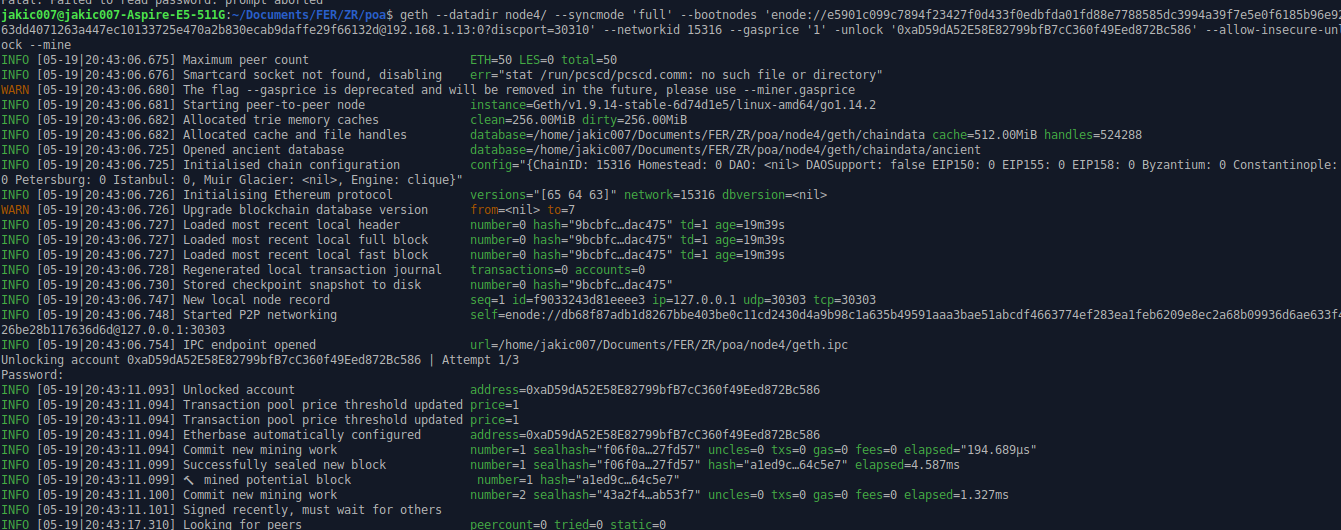
\includegraphics[width=\textwidth]{nodeStart.png}
  \caption{Ispis nakon pokretanja geth procesa}
  \centering
\end{figure}

Iz ispisa se može vidjeti kako je nakon upisane lozinke za otključavanje novčanika pokrenuto rudarenje, odnosno kreiranje blokova.
Potrebno je imati (N/2)+1 čvorova \emph{online} kako bi se blokovi
kontinuirano stvarali gdje je N broj adresa navedenih u \emph{genesis.json} datoteci. U slučaju da neki čvor \emph{ispadne},
blokovi će se stvarati dokle god je dovoljno aktivnih čvorova. Kad se čvor ponovno poveže, on će uskladiti svoje stanje
s ostalima kako bi povijest bila svugdje jedinstvena. \\
Novi blok se generira svako 15 sekundi jer je tako zadano prilikom inicijalizacije \emph{genesis.json} datotekom. \\
U isto se vrijeme na \emph{bootnodeu} vide \emph{ping-pong} poruke čvorova što znači da su svi čvorovi uspješno povezani i međusobno
vidljivi.

\begin{figure}[ht]
  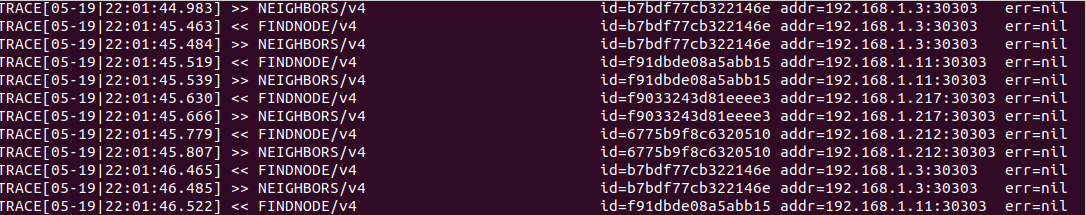
\includegraphics[width=\textwidth]{bootnode.png}
  \caption{Komunikacija čvorova i \emph{bootnodea}}
  \centering
\end{figure}

\pagebreak
\section{Praćenje stanja (engl. \emph{monitoring})}
U prijašnjem odjeljku je pokrenuta potpuno funkcionalna mreža no korisnicima nije jednostavno pratiti stanje gledajući
dnevnike (engl. \emph{logs}) iz komandne linije. Postoji mnogo besplatnih dostupnih i otvorenih alata koji nude jednostavniji
prikaz bitnih podataka u obliku jednostavne web aplikacije koja se povezuje izravno na čvor. Obično se koristi http protokol
ili websocket veza kako bi se podaci dobavljali.
\subsection{Pretražitelj blokova (engl. \emph{block explorer})}
Osnovni dio praćenja stanja je \emph{block explorer}. Pomoću njega se može u realnom vremenu pratiti stanje \emph{blockchaina}
što podrazumijeva prikaz najvišeg trenutnog bloka (engl. \emph{block height}) te pretraživanje i filtriranje transakcija u 
pojedinom bloku. \\
Odabrana je aplikacija \emph{Alethio Ethereum Lite Explorer}\footnote{\url{https://aleth.io/products/explorer}} zbog svoje jednostavnosti i ažurnosti. To je klijentska
web aplikacija koja se povezuje na bilo koji \emph{Ethereum} čvor koji ima omogućen udaljen poziv procedura (engl. \emph{RPC}).\citep{explorer} \\
Čvorovi postavljeni u prethodnom dijelu nemaju omogućen udaljen poziv procedura. Da ga omogućili potrebno je zaustaviti geth proces
na odabranom uređaju te ponovno pokrenuti dodavanjem parametara:

\begin{lstlisting}
  --rpc --rpcaddr 'localhost' --rpcport 8545  --rpcapi 'personal,db,eth,net,web3,txpool,miner' --rpccorsdomain "*"
\end{lstlisting}

Ovim postupkom je omogućeno spajanje bilo kojeg servisa s istog računala na naš \emph{geth} proces putem porta 8545 i http protokola.

Postoje dva načina pokretanja ove aplikacije, prevođenjem izvornog koda na vlastitom računalu ili već javno dostupnim
\emph{docker} kontejnerom. Zbog jednostavnosti i niske zahtevnosti, za ovaj projekt je odabran drugi način.
Jedini preduvjet je imati instaliran \emph{docker} klijent na računalu. Nakon toga se sve pokreće jednom naredbom.

\begin{lstlisting}
  $ docker run -p 8080:80 -e APP_NODE_URL="http://localhost:8545" alethio/ethereum-lite-explorer
\end{lstlisting}

\emph{Docker} provjerava postoji li već lokalno dostupna slika te ako ne postoji je dohvaća s \emph{Docker Hub}\footnote{\url{https://hub.docker.com/}} repozitorija.
Ovim načinom nije potrebno mijenjati konfiguracijsku datoteku već je dovoljno samo dodati varijablu okoline (engl. \emph{environment variable})
koja aplikaciji daje IP adresu i vrata čvora na koji se potrebno spojiti. \\
Parametrom "-p 8080:80" se prosljeđuje \emph{port} 80 unutar kontejnera na \emph{port} 8080 na uređaju na kojem se pokreće kontejner. \\
Utipkavanjem adrese "localhost:8080" u željeni preglednik otvara se aplikacija i prikazuje početni ekran. \\
Blok 47 na slici je prazan, odnosno niti jedna transakcija se nije dogodila u njemu.

\begin{figure}[ht]
  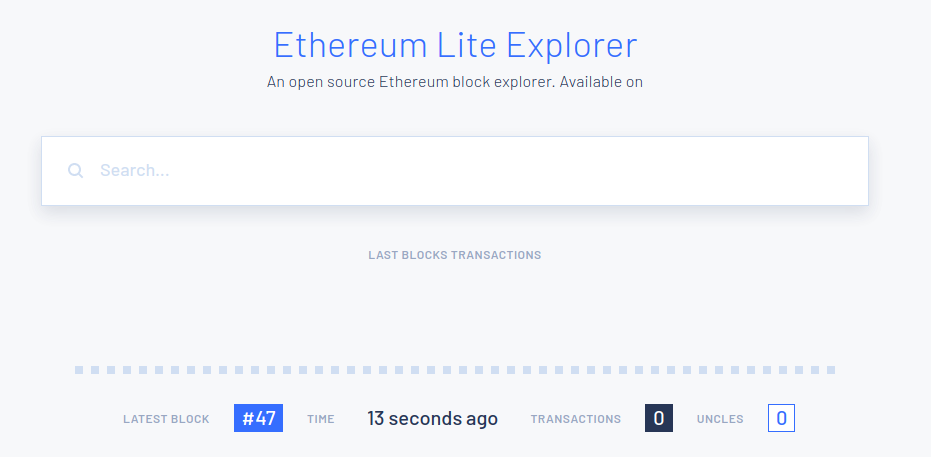
\includegraphics[width=\textwidth]{blockexplorer.png}
  \caption{Početni ekran pretražitelja blokova}
  \centering
\end{figure}

\subsection{Opterećenost čvorova}
Za dobivanje podataka potrebnih za usporedbu performanci na raznorodnom sklopovlju potreban je poseban servis koji će pratiti
opterećenost sklopovlja čvora. Jednako kao i za praćenje stanja blokova, postoji više dostupnih alata. Za ovaj rad je ponovno
odabran \emph{Alethiov} alat \emph{ethstats}\footnote{\url{https://ethstats.io/}}. Razlog tome je što je jedini redovno održavan, besplatan i moguće ga je pokrenuti
uz vrlo malo konfiguracije pomoću \emph{docker-composea}. \\
Dovoljno je preuzeti datoteku s poveznice
 \footnote{\url{https://raw.githubusercontent.com/Alethio/ethstats-network-server/master/docker/lite-mode/redis-persistence/docker-compose.yml}} koju 
 treba izmijeniti za ovu konfiguraciju. \\
\emph{Ethstats} se sastoji od više servisa koji čine cjelinu. \emph{Docker-compose} nam olakšava pokretanje te nakon podešavanja
varijabli okruženja unutar \emph{docker-compose.yaml} datoteke moguće je pokrenuti sve servise jednom naredbom.
\begin{lstlisting}
  $ docker-compose up -d
\end{lstlisting}
Time smo pokrenuli \emph{ethstats server}, \emph{dashboard}, \emph{redis} i \emph{deepstream}.
Server pribavlja podatke s čvorova i sprema ih u \emph{Redis} bazu podataka i istovremeno pruža \emph{dashboardu} i \emph{deepstreamu} koji
su zaduženi za grafički prikaz i analitiku. \\
Pokretanjem prethodne naredbe dobiva se pogreška koja kaže da se server ne može povezati na \emph{ethstats-cli}. \emph{ethstats-cli} 
je odvojeni servis koji se treba pokrenuti na svakom čvoru koji se želi pratiti. On je zaslužan za prikupljanje podataka o iskorištenosti
memorije, procesora i ostalih detalja o sklopovlju. Njegov zahtjev je prethodno instaliran \emph{node} verzije novije od 8.11 što se može 
provjeriti naredbom:
\begin{lstlisting}
  $ node -v
\end{lstlisting}
Kad je osigurana odgovarajuća verzija \emph{nodea} moguće je globalno instalirati \emph{ethstats-cli} i pokrenuti naredbama:
\begin{lstlisting}
  $ npm install -g ethstats-cli
  $ ethstats-cli --server-url http://192.168.1.217:3000 -r --account-email jakov.buratovic@fer.hr --node-name pc
\end{lstlisting}
Prvim pokretanjem obavlja se registracija čvora pa je zbog toga unesena adresa e-pošte i proizvoljan naziv čvora. IP adresa u argumentu
"--server-url" jest IP adresa računala na kojem će biti pokrenut \emph{ethstats-server}. U ovom primjeru je to prijenosno računalo. \\
Sada možemo izmijeniti \emph{docker-compose.yaml} datoteku željenim uređivačem teksta. Dovoljno je promijeniti konfiguraciju servisa
\emph{server} na sljedeći način:
\begin{lstlisting}
  server:
    container_name: ethstats-network-server
    image: alethio/ethstats-network-server:latest
    restart: always
    depends_on:
      - deepstream
      - redis
    ports:
      - 127.0.0.1:3000:3000
      - 192.168.1.217:3000:3000
      - 127.0.0.1:3030:3030
      - 127.0.0.1:8888:8888
    environment:
      - NETWORK_ID=15316
      - NETWORK_NAME=dev
\end{lstlisting}

U odnosu na zadanu konfiguraciju, dodano je preusmjeravanje unutarnjeg porta 3000 na vanjsko sučelje računala kako bi ostali uređaji
u lokalnoj mreži mogli vidjeti \emph{ethstats-server} te je izmijenjen identifikator mreže koji je bio postavljen na vrijednost "1" što
označava glavnu Ethereum mrežu, \emph{Ethereum mainnet}. Ako ponovno pokrenemo \emph{docker-compose} trebali bismo uspješno biti povezani
na čvorove i posjetom adrese "localhost:80" bit će prikazano sučelje.

\begin{figure}[ht]
  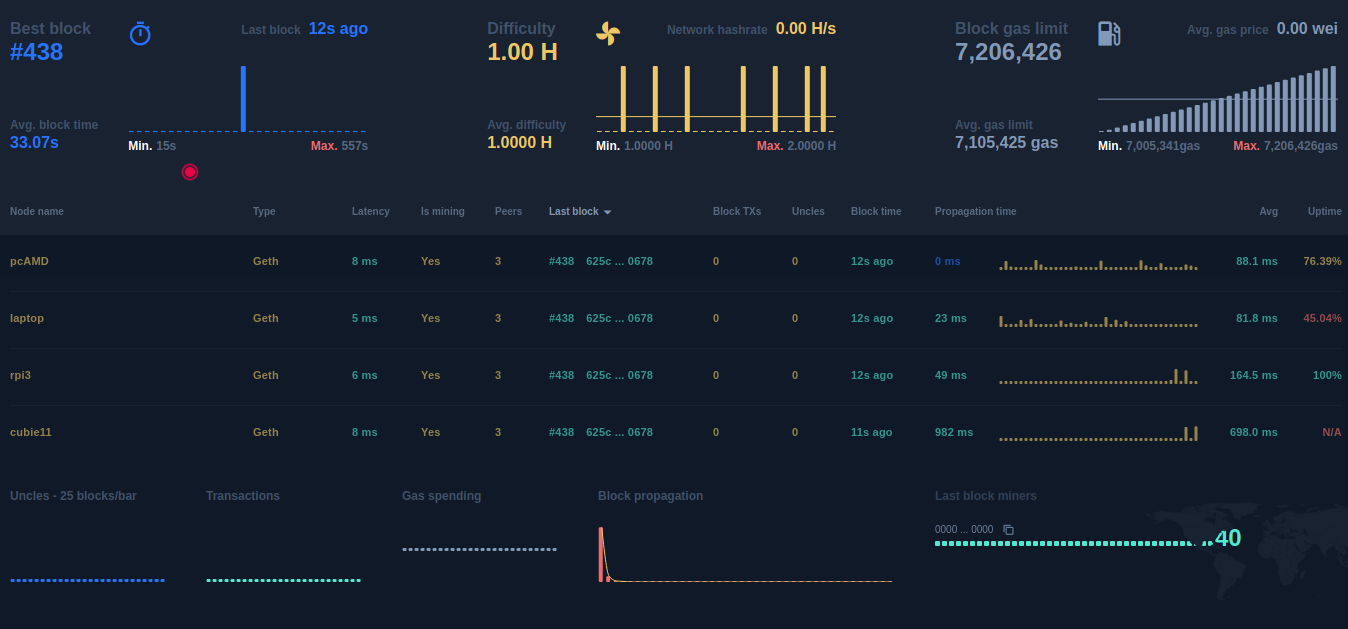
\includegraphics[width=\textwidth]{ethstatsDashboard.png}
  \caption{Sučelje \emph{ethstatsa}}
  \centering
\end{figure}

Kao i u \emph{block exploreru} vidljiv je posljednji blok no ovoga puta uz više detalja i podacima za svaki čvor posebno.
Desno od posljednjeg bloka vidimo statistiku o vremenu kreiranju novih blokova. Minimalno vrijeme je 15 sekundi što odgovara konfiguraciji
no maksimalno vrijeme je 557 sekundi što znači da 557 sekundi nije bilo dovoljno povezanih čvorova u mreži i proizvodnja blokova je stala. \\
Ispod vidimo listu svih čvorova s osnovnim podacima kao što su brzina odaziva, broj povezanih čvorova na taj čvor, posljednji blok na pojedinom
čvoru te brzinu propagiranja novog bloka na čvoru. \\
Iz ove liste vidimo da su svi čvorovi sinkronizirani na istom posljednjem bloku što nam govori da je njihovo sklopovlje dovoljno sposobno
pokretati ovakav tip mreže. Veće opterećenje se može postići skraćivanjem vremena kreiranja blokova i izvršavanjem složenih programskih
kodova pametnih ugovora. \\
Za više detalja potrebno je odabrati čvor čime se otvara novi prikaz u kojem vidimo zauzeće procesora i radne memorije u odabranom
 razdoblju.
\pagebreak

\begin{figure}[ht]
  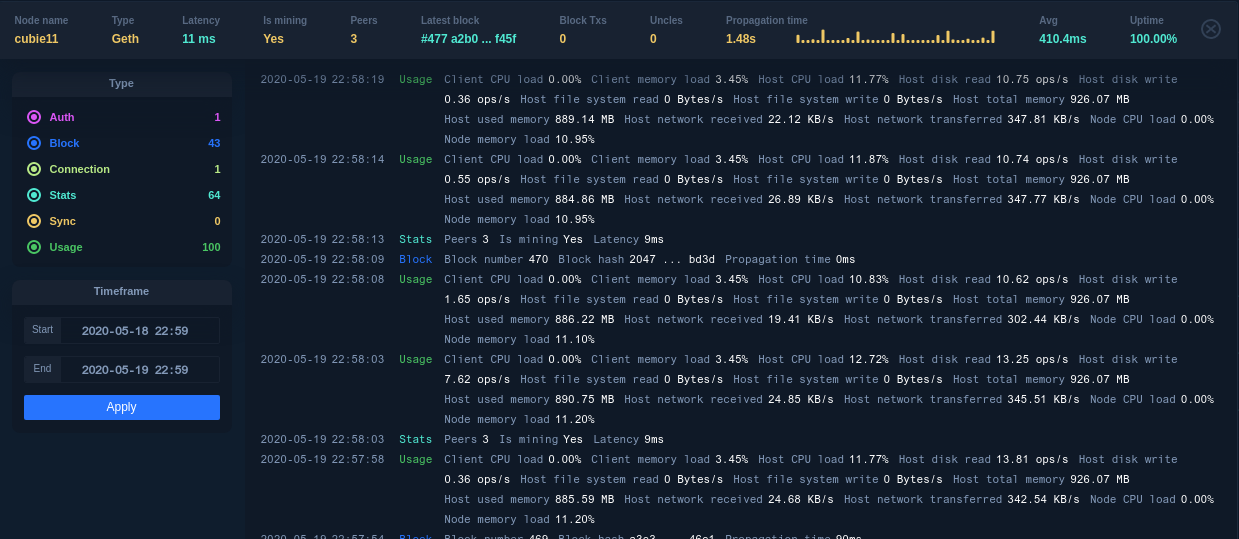
\includegraphics[width=\textwidth]{ethstatsCubie.png}
  \caption{Opterećenost Cubieboard2 pločice}
  \centering
\end{figure}

\emph{Ethstats} je odlično rješenje za nadgledanje više sustava na jednom računalu preko jedinstvenog sučelja. Ako želimo najpreciznije 
moguće podatke u stvarnom vremenu onda je potrebno na pojedinom uređaju pokrenuti neki servis za nadgledanje iskorištenosti resursa kao
na primjer \emph{htop} koji je predinstaliran u većini distribucija \emph{Linuxa} i pokreće se izravno iz terminala. Na grafu niže
je zabilježena prosječna opterećenost procesora na pojedinom uređaju procesom \emph{geth}. Kao što je vidljivo za moderno stolno ili prijenosno računalo opterećenost
je gotovo zanemariva dok se na \emph{single-board} računalima proces pokazao nešto zahtjevniji. Raspberry Pi 1 jedini na ovom grafu ne bi trebalo izravno uspoređivati
jer njegov \emph{geth} proces nije obavljao jednak zadatak kao i na ostalim čvorovima. On nije uopće sinkronizirao blokove niti sudjelovao u njihovom stvaranju nego
je samo služio kao središnja jedinica za pronalaženje čvorova u mreži. S obzirom na to da njegovo sporije sklopovlje, čak i s tim zadatkom je bio najviše opterećen.

\begin{figure}[ht]
  \caption{Iskorištenost procesora}
  \centering
  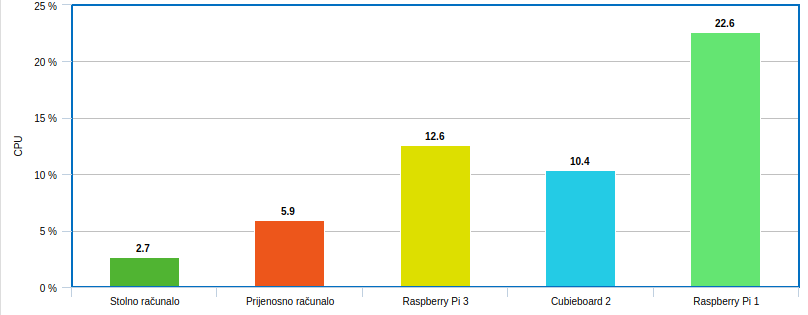
\includegraphics[width=\textwidth]{cpuUtil.png}
\end{figure}

\emph{Htop} nam pruža precizne podatke i o postotku zauzeća radne memorije pojedinim procesom. Ovdje je jasno vidljivo kako je Raspberry Pi 1 imao manje zahtjevan
zadatak te unatoč njegovih 192 MB dostupne memorije, samo je otprilike 20 MB zauzeto \emph{geth} procesom dok na uređajima koji moraju pratiti stanje na \emph{blockchainu}
proces zahtjeva više memorije. Ponovno, za modernija računala ti zahtjevi nisu visoki dok bi na \emph{single-board} računalima memorija mogla predstavljati usko grlo
u nekom složenijem sustavu s više pokrenutih procesa u isto vrijeme.

\begin{figure}[ht]
  \caption{Iskorištenost memorije}
  \centering
  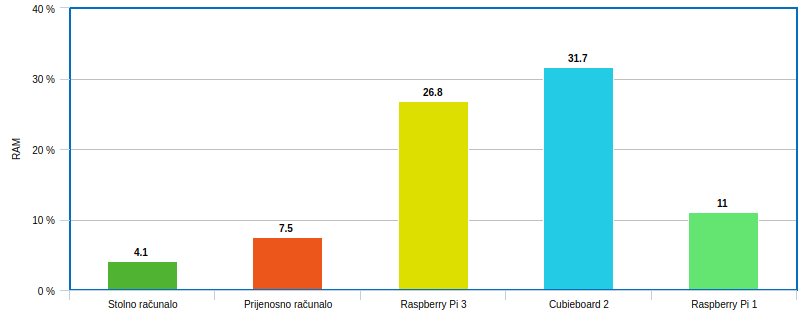
\includegraphics[width=\textwidth]{ramUtil.png}
\end{figure}

\section{Transakcije i pametni ugovori}
Sama mreža nije pretjerano korisna dok su blokovi prazni, odnosno dok se ne odvijaju nikakve transakcije među članovima mreže. Transakcije mogu biti vrlo jednostavne
kao na primjer slanje određene količine \emph{Ethera} s jednog novčanika na drugi ili složenije kao postavljanje programskog koda u obliku pametnog ugovora ili interakcija
s već postavljenim pametnim ugovorom te izvršavanje njegovog koda. \\
Korisnik ima više različitih dostupnih načina izvršavanja transakcija. Najprimitivniji način i isto tako rijetko korišten od strane korisnika jest interakcija putem
naredbenog retka koristeći \emph{geth cli}. Taj način zahtjeva dobro znanje o naredbama i razumijevanje njihovih akcija. \\
Osim naredbenog retka, postoje brojne aplikacije koje se mogu povezati na mrežu putem biblioteke te na način prilagođen njenim zahtjevima nuditi određene mogućnosti
interakcije. Najčešće su te aplikacije pisane u \emph{Javascriptu} i koriste \emph{web3.js}\footnote{\url{https://web3js.readthedocs.io/en/v1.2.8/#}} biblioteku zbog
jednostavne integracije s web aplikacijama za preglednike i vrlo dobre dokumentacije.
Za ovaj rad je odabran \emph{Metamask}\footnote{\url{https://metamask.io/}}, klijentska aplikacija za upravljanje novčanicima i izvođenje i potpisivanje transakcija. 
Dostupna je kao ekstenzija za \emph{Chromium} i \emph{Firefox} preglednike ili kao mobilna \emph{iOS} ili \emph{Android} aplikacija. 
\subsection{Slanje i primanje Ethera}
Nakon instalacije \emph{Metamask} aplikacije u preglednik, otvara se njeno sučelje te traži korisnika da izradi novi novčanik ili se prijavi s postojećim.
Kako su prethodno već generirani novčanici koje koriste čvorovi, potrebno je njih ubaciti. Da bismo ubacili postojeći novčanik u \emph{Metamask} potrebno je znati ili
privatni ključ novčanika ili koristiti \emph{json} datoteku koja je automatski izrađena prilikom generiranja novčanika \emph{gethom}. Tajna datoteka se nalazi
u pod direktoriju \emph{keystore}.

\begin{figure}[ht]
  \centering
  \begin{minipage}[b]{0.4\textwidth}
    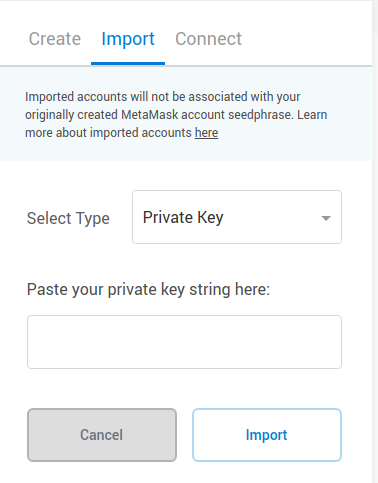
\includegraphics[width=\textwidth]{mmimportprivate.png}
    \caption{Prijava privatnim ključem}
  \end{minipage}
  \hfill
  \begin{minipage}[b]{0.4\textwidth}
    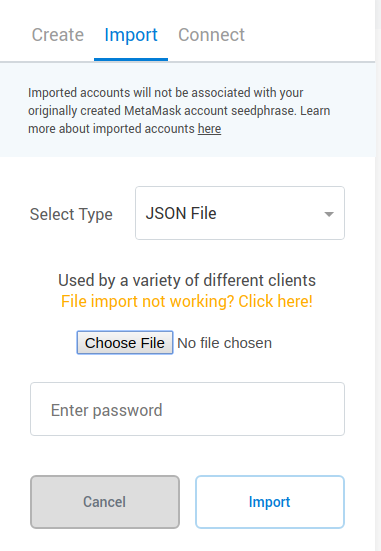
\includegraphics[width=\textwidth]{mmiportjason.png}
    \caption{Prijava datotekom}
  \end{minipage}
\end{figure}

Nakon što je \emph{Metamask} uspješno postavljen novčanikom može se vidjeti da je trenutno stanje 0 ETH. Razlog tome je što je \emph{Metamask} inicijalno povezan
na glavnu \emph{Ethereum} mrežu, \emph{mainnet}. Potrebno je podesiti aplikaciju da bude povezana na neki od čvorova privatne mreže. Treba odabrati \emph{Localhost 8545}
jer je čvor na računalu s \emph{Metamask} klijentom dostupan preko unaprijed zadanog porta 8545. 

\pagebreak

\begin{figure}[ht]
  \centering
  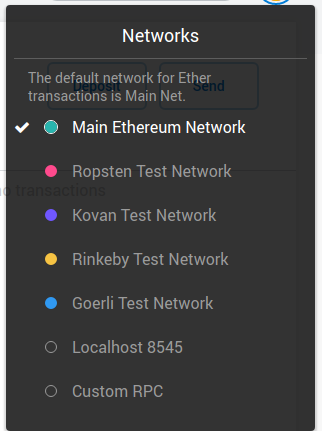
\includegraphics[scale=0.5]{mmnetworkdd.png}
  \caption{Odabir mreže}
\end{figure}

Ako se \emph{Metamask} uspješno povezao na čvor, pisat će stanje na novčaniku. To stanje odgovara inicijalnom stanju zadanom u \emph{genesis.json} datoteci ako
nisu već provedene transakcije. Kako je u ovom primjeru zadana vrlo visoka vrijednost koja u primjerice glavnoj mreži ne bi uopće bila moguća, prikaz nije idealno
formatiran no to neće umanjiti funkcionalnosti.

\begin{figure}[ht]
  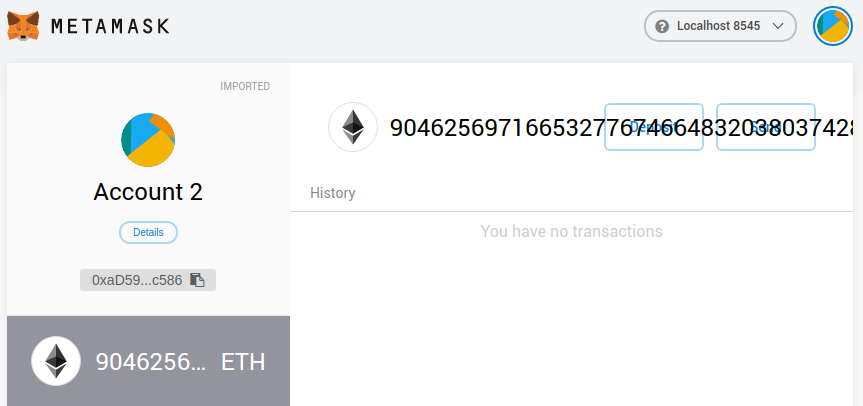
\includegraphics[width=\textwidth]{mmimported.png}
  \caption{Stanje}
  \centering
\end{figure}

Odabirom gumba \emph{Send} otvara se novi prikaz u koji je moguće upisati adresu novčanika primatelja i željeni iznos za transakciju. Ispod polja za upis iznosa
postoji mogućnost odabira provizije koja će biti utrošena prilikom provedbe transakcije. U \emph{proof of authority} ta opcija nije važna, odnosno nema razlike u brzini
izvođenja transakcije. Najbolje je odabrati najnižu vrijednost ili upisati ručno. Te vrijednosti su zanemarive u odnosu na stanje koje je na novčaniku tako da niti veća
provizija neće biti značajna u ovom slučaju. Provizija se dijeli čvorovima u mreži koji su navedeni u \emph{genesis.json} datoteci te tako ostaje u cirkulaciji.

\begin{figure}[ht]
  \centering
  \begin{minipage}[b]{0.4\textwidth}
    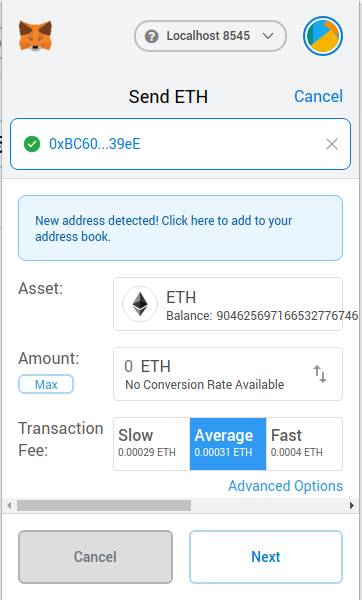
\includegraphics[width=\textwidth]{mmsendtocubie.png}
    \caption{Slanje transakcije}
  \end{minipage}
  \hfill
  \begin{minipage}[b]{0.4\textwidth}
    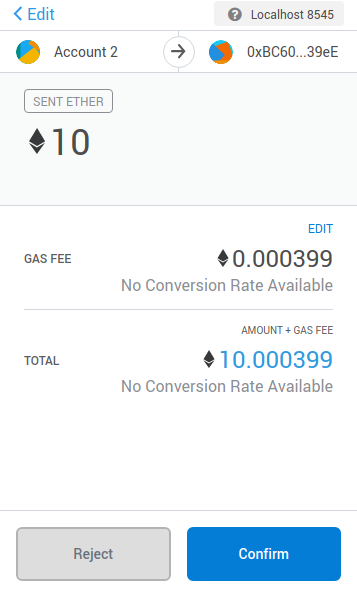
\includegraphics[width=\textwidth]{sent.png}
    \caption{Pregled i potvrda}
  \end{minipage}
\end{figure}

Nakon što je transakcija poslana ona se objavljuje čvoru koji ju provjerava i potom uključuje u idući blok, daje joj identifikator i propagira ju ostalim čvorovima.
U najviše 15 sekundi bi se novi blok trebao stvoriti s tom transakcijom. To će biti jasno vidljivo u pretražitelju blokova. Odabirom bloka i transakcije u njemu se otvara 
prikaz detalja o toj transakciji kao što su identifikator, adrese primatelja i pošiljatelja, iznos koji je poslan i provizija koja je utrošena. U gornjem dijelu postoji
informacija o broju potvrda. To je podatak koji govori koliko je blokova generirano nakon bloka s tom transakcijom.

\pagebreak

\begin{figure}[ht]
  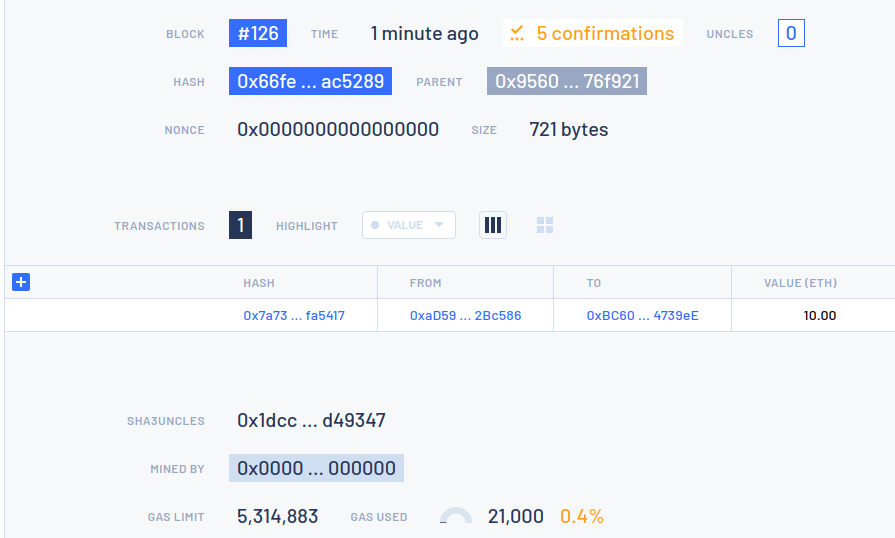
\includegraphics[width=\textwidth]{blocktx.png}
  \caption{Prva transakcija}
  \centering
  \vfill
\end{figure}

\subsection{Pametni ugovori}
Pametni ugovori su ono što \emph{Ethereum} razlikuje od običnih kriptovaluta koje služe samo za razmjenu vrijednosti putem transakcija. Danas postoji velik broj postavljenih 
pametnih ugovora na glavnoj \emph{Ethereum} mreži. Postavljanje pametnog ugovora je transakcija kojom se šalje prevedeni kod pametnog ugovora na \emph{blockchain}.
Kod se piše u objektno orijentiranom jeziku \emph{Solidity} i prevodi koristeći \emph{solc}\footnote{\url{https://www.npmjs.com/package/solc}}, prevoditelj za Solidity. Prevođenjem programskog koda dobiva se binarna datoteka
i aplikacijsko binarno sučelje (engl. \emph{ABI - application binary interface}). \emph{ABI} služi kao sučelje za interakciju s pametnim ugovorom. Nakon što je kod
proveden potrebno je postaviti produkte prevođenja na \emph{blockchain}.
\subsubsection{Kod i prevođenje}
Najjednostavniji način za isprobati \emph{Solidity} i pametne ugovore je koristeći službeni \emph{Ethereumov IDE Remix}\footnote{\url{https://remix.ethereum.org/}}. 
To je web aplikacija koja se također može povezati na bilo koji \emph{Ethereum} čvor ali i naravno na glavnu mrežu u kojoj je moguće pisati programski kod
pametnih ugovora u \emph{Solidity} programskom jeziku. Iz iste aplikacije je moguće korištenjem ugrađenih dodataka prevesti taj kod i postaviti ga na mrežu.
Upravo iz tog razloga je idealan alat za brzo isprobavanje ili testiranje pametnih ugovora jer nije potrebno postavljati kompleksna razvojna okruženja. \\
Otvaranjem početne stranice, s lijeve strane je prikazan pretražitelj datoteka. Tu se nalazi nekoliko jednostavnih primjera pametnih ugovora koji su dovoljni
za demonstriranje samog toka događaja pa iz tog razloga za ovaj rad nije pisan nikakav kompleksniji kod. \emph{Solidity} datoteke imaju nastavak \emph{.sol}
pa ih je lako prepoznati. \\
Za ovaj rad će se koristiti prvi primjer \emph{1\_Storage.sol} pa ga je potrebno otvoriti s dva klika kako bi se prikazao njegov izvorni kod.
U prvoj liniji koda definirane su valjane verzije \emph{Solidity} jezika u kojima će se ovaj kod moći uspješno prevesti. To je vrlo važno jer je jezik
nov i vrlo brzo izlaze nova izdanja koja mijenjaju bitne stvari pa iz tog razloga starija sintaksa neće biti valjano prevedena s novijim prevoditeljem. Također je moguće
navesti raspon verzija kao što je u ovom primjeru stavljeno. \\
Nakon definiranja verzije, ključnom riječi \emph{contract} definira se naziv ugovora. Kako je \emph{Solidity} objektno orijentiran jezik, ta ključna riječ odgovara 
riječi \emph{class} u primjerice \emph{Java} jeziku. Unutar tijela ugovora se definiraju metode i varijable. Metode mogu biti označene s ključnom riječi \emph{view} što
znači da ta metoda ne upisuje ništa na \emph{blockchain} nego samo pribavlja i čita podatke s njega. Izvođenje takvih metoda je besplatno za razliku od metoda koje
upisuju podatke. Svako upisivanje na \emph{blockchain} zahtjeva transakciju koja mora biti uključena u blok što košta. \\
Ovaj ugovor ima dvije vrlo jednostavne metode. Jedna metoda upisuje broj na \emph{blockchain}, a druga vraća posljednji upisan broj. 
Varijabla \emph{uint256 number} je varijabla koja je pohranjena u memoriji samog ugovora. Metoda \emph{store} prima kao argument \emph{uint256} broj koji postavlja 
varijablu ugovora na unesenu vrijednost. \\
Nakon što je kod napisan potrebno je s lijeve strane odabrati \emph{Solidity compiler} dodatak koji služi za prevođenje koda. U prikazu se odabire verzija prevoditelja
i ugovor koji korisnik želi prevesti. Odabirom gumba \emph{Compile 1\_Storage.sol}, ugovor je uspješno preveden.

\begin{figure}[ht]
  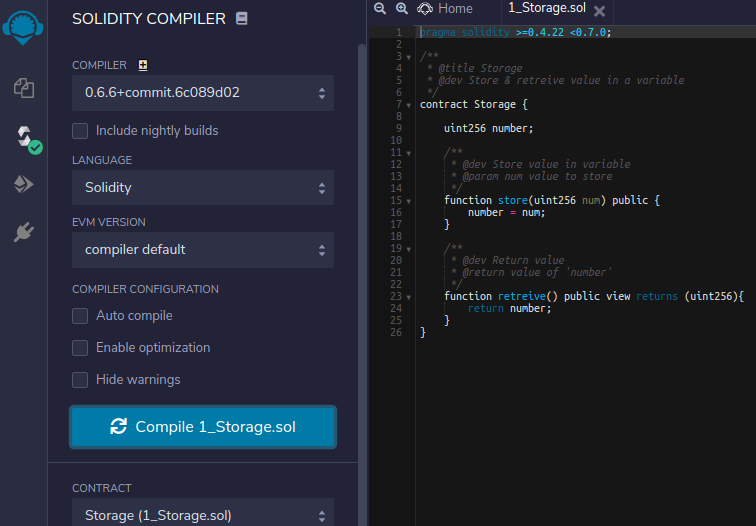
\includegraphics[width=\textwidth]{remixcompiled.png}
  \caption{Prevođenje pametnog ugovora}
  \centering
  \vfill
\end{figure}

\pagebreak

Dobivene produkte prevođenja treba postaviti na \emph{blockchain}. U izborniku s lijeve strane treba odabrati dodatak \emph{Deploy and run transactions} što otvara
prikaz u kojem se odabire okolina. Ako u izborniku nije dostupan taj dodatak potrebno je odabrati posljednju stavku u izborniku, upravitelj dodacima (engl. \emph{Plugin manager})
u čije s polje za pretraživanje može upisati ključna riječ \emph{deploy} i aktivirati dodatak pritiskom na gumb \emph{activate}.
Dostupne su tri okoline, \emph{Javascript VM, Injected Web3} i \emph{Web3} provider. \\
\emph{Javascript VM} je virtualni stroj koji se izvodi u pregledniku i ne spaja se na stvarne čvorove. To je dobra opcija za testiranje ispravnosti koda prije postavljanja
na mrežu. Za potrebe ovog rada može poslužiti bilo koja od preostale dvije opcije. Odabirom \emph{Web3 Provider} opcije, \emph{Remix} se izravno spaja na čvor dok odabir
\emph{Injected Web3} opcije podrazumijeva da korisnik ima postavljen \emph{Metamask} ili neki drugi novčanik u pregledniku koji onda upravlja pozivima i transakcijama.
Ako je odabran \emph{Web3 Provider} onda treba u istom prikazu odabrati \emph{Ethereum} račun koji će se koristiti za postavljanje ugovora i ograničenje potrošnje
\emph{gasa}. U slučaju da se koristi \emph{Metamask}, otvara se novi prozor u kojem se od korisnika traži dozvola korištenja \emph{Metamaska} od strane \emph{Remixa}.
Račun i ograničenje \emph{gasa} se podešavaju u istom prozoru nakon odabira gumba \emph{Deploy} u \emph{Remixu}. 

\begin{figure}[ht]
  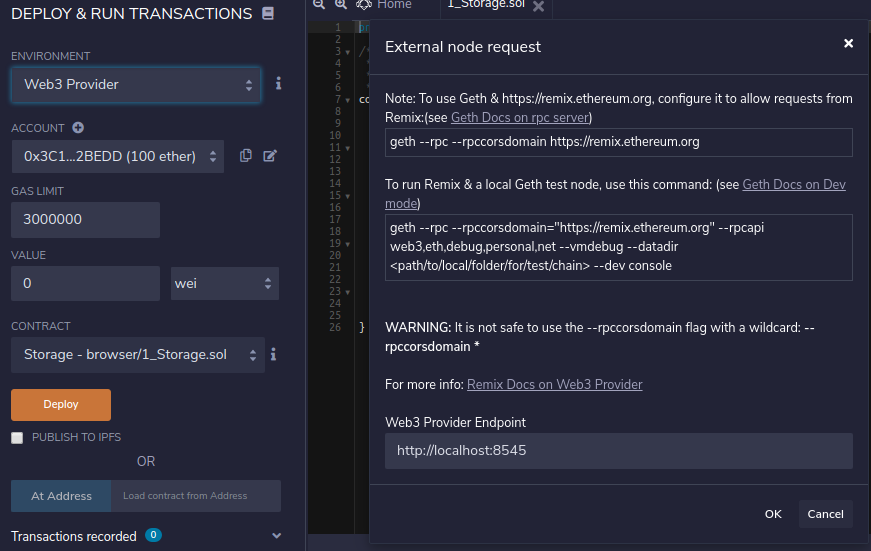
\includegraphics[width=\textwidth]{remixconnect.png}
  \caption{Postavljanje ugovora}
  \centering
  \vfill
\end{figure}

U idućem bloku je uključena transakcija koja kreira ugovor na jedinstvenoj adresi, odnosno ugovor posjeduje svoj novčanik čiji je vlasnik sam ugovor. 
U ovom trenutku je moguće izvršavati programski kod ugovora s bilo kojeg člana mreže jer se on replicirao na svaki čvor prilikom sinkronizacije posljednjeg bloka.
Vrijednosti varijabli i rezultati izvršavanja metoda ugovora su također usklađeni u svakom čvoru što je vrlo korisna funkcionalnost. Nitko ne može mijenjati stanje
bez da to svi ostali znaju. \\
U \emph{Remixu} se pojavljuje novi izbornik koji služi za pozivanje metoda postavljenog ugovora. Vidi se metoda \emph{store} i \emph{retreive}. Kao što je i napisano
u kodu, prva metoda prima broj tipa \emph{uint256} te ga postavlja u varijablu pametnog ugovora u idućem bloku. Ta se transakcija plaća vrlo malim iznosom \emph{gasa}
jer je to operacija upisivanja na \emph{blockchain}. Operacija \emph{retrieve} je operacija čitanja što znači da se ona neće pojaviti kao transakcija i potpuno je 
besplatna. 

\pagebreak

\begin{figure}[ht]
  \centering
  \begin{minipage}[b]{0.4\textwidth}
    \includegraphics[width=\textwidth]{remixfunctions.png}
    \caption{Raspoložive metode}
  \end{minipage}
  \hfill
  \begin{minipage}[b]{0.4\textwidth}
    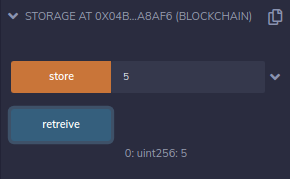
\includegraphics[width=\textwidth]{number5retreived.png}
    \caption{Dohvaćanje vrijednosti}
  \end{minipage}
\end{figure}

\subsubsection{Primjer složenijeg ugovora}

U ovom ugovoru je dozvoljeno bilo kome mijenjati vrijednost varijable. U nekim slučajevima to je željena mogućnost. Za neku drugu funkcionalnost je možda poželjno da
samo određeni računi smiju upisivati, a svi ostali čitati. Dobar primjer malo složenijeg ugovora je lutrija. \\
Jednostavan primjer ugovora za lutriju bi dozvoljavao da bilo tko može igrati, odnosno uložiti \emph{Ether} na adresu pametnog ugovora ali da nitko ne može pokrenuti
izvlačenje sretnog dobitnika osim vlasnika ugovora, odnosno računa koji je postavio ugovor na \emph{blockchain}. Pokretanjem metode za izvlačenje dobitnika nasumično
se bira jedna adresa novčanika iz liste svih koji su sudjelovali u tom krugu lutrije te se njemu isplaćuje cjelokupan sadržaj novčanika ugovora. Nakon toga se lista
novčanika prazni i kreće novi krug lutrije. \\
Ugovor bi bio još bolji kad bi se potpuno izbacio utjecaj vlasnika jer igrači nemaju nikakvu garanciju da će vlasnik ikada pokrenuti izvlačenje. To se može napraviti
tako da se u kodu napiše da se izvlačenje pokreće samostalno primjerice kad je dovoljan broj različitih novčanika igrao ili kad je dostignuto dovoljno stanje na računu
samog ugovora.

\chapter{Zaključak}
\emph{Ethereum} je samo jedan primjer mreže temeljene na tehnologiji distribuirane knjige. Za ovaj rad je bilo prigodno osloniti se na \emph{Ethereum} zbog 
velike količine dostupne javno dostupne dokumentacije i besplatnih alata. Osim toga, modularnost \emph{Ethereuma} je omogućila korištenje protokola s različitim
algoritmima konsenzusa za različite potrebe. Bez obzira na algoritam konsenzusa, funkcionalnost platforme ostaje nepromijenjena.
To je idealno svojstvo za ovaj primjer jer \emph{proof of work} algoritam ne bi bilo moguće izvoditi na jeftinijem i slabijem sklopovlju zbog svoje implementacije
koja zahtjeva velik utrošak energije za validiranje transakcija i blokova. \emph{Proof of authority}
algoritam je prigodan za uređaje niske potrošnje i zatvorene sustave u kojima je potrebna brža distribucija informacija po mreži i gdje su sudionici mreže poznati i 
provjereni. \\
Samo postavljanje mreže nije zahtjevno, ali pretpostavlja osnovno razumijevanje mrežnih protokola, arhitekture računala i specifikacije \emph{Ethereuma}. 
U ovom radu je pokazano kako gotovo bilo tko može pokretati vlastiti čvor koji će biti uključen u mrežu iz vlastitog doma na postojećem računalu ili 
\emph{single board} računalu. Osim toga, nije potrebno osigurati računalo specifično za taj proces, već je moguće paralelno koristiti računalo za rad i svakodnevne poslove
dok se u pozadini izvršava proces čvora i sinkronizira podatke. Također, nije potrebno niti biti na mreži konstantno jer se ponovnim uključivanjem u mrežu povijest
sinkronizira s ostalim čvorovima. Trebalo bi provjeravati zauzeće memorije za pohranu. Stvaranjem blokova se 
upisuju novi podaci na svaki čvor mreže te oni čuvaju cjelovitu povijest u svojoj lokalnoj bazi podataka. Primjerice, u glavnoj mreži \emph{Ethereuma} veličina
podataka u bazi godišnje poraste za oko 75 GB. S obzirom na to da je dovoljna i sporija memorija za pohranu, nije potrebno ulagati u brže \emph{SSD} komponente za pohranu jer
je i obični čvrsti disk dovoljno dobro rješenje. \\
Ova tehnologija je još uvijek u razvoju i nije dostigla razinu adopcije kao primjerice internet. Smatram da ulaganjem u obrazovanje i širenjem svijesti o novim mogućnostima
udaljene komunikacije ova tehnologija može donijeti velike prednosti u raznim djelatnostima koje zahtjevaju dodatnu razinu sigurnosti i pouzadnosti. 

\bibliography{literatura}

\bibliographystyle{fer}

\begin{sazetak}
Proučiti i objasniti osnove tehnologije raspodijeljene glavne knjige i najpoznatije algoritme konsenzusa koji se primjenjuju danas. Usporediti njihove prednosti i 
mane. \\
Dati kratak prikaz povijesti i arhitekture \emph{Ethereum} mreže te pojasniti kako se odvijaju transakcije i izvršava programski kod.\\
Proučiti mogućnost postavljanja privatne mreže u svrhu testiranja izvođenja transakcija i koda pametnih ugovora na vlastitom sklopovlju različite procesorske arhitekture
i snage. Postaviti mrežu i testirati dodatne funkcionalnosti koje približavaju ovu simulaciju stvarnoj uporabi.

\kljucnerijeci{raspodijeljena glavna knjiga, algoritmi konsenzusa, pametni ugovori, decentralizirani sustav, transakcije, čvorovi}
\end{sazetak}

% TODO: Navedite naslov na engleskom jeziku.
\engtitle{Performance Comparison of the Ethereum Blockchain on Heterogeneous Hardware}
\begin{abstract}
Analyze and describe basics of the Distributed Ledger Technology and well known consensus algorithms that are used today. Compare their pros and cons. \\
Give short review of history and architecture of the \emph{Ethereum} network and explain execution of transactions and program instructions. \\
Examine the possibility of setting up a private network for the purpose of testing and executing transactions and smart contracts on your own hardware with different 
architecture and power. Set up a network and test additional functionalities that bring this simulation closer to actual use. 

\keywords{Distributed Ledger Technology, consensus algorithms, smart contracts, decentralized system, transactions, nodes}
\end{abstract}

\end{document}
